\section{Introduction}

In the previous chapter, we presented an initial model to reduce the carbon emissions of operating a cloud federation for the short term (one year) by sizing its renewable infrastructure, that is, defining the area of solar panels and the capacity of the batteries for each data center. Given that the cloud federation will operate for the long term, the decision-maker needs to be sure of the investments that will be made to avoid wasting money and generating environmental impact with a bad strategy. Furthermore, a planning process is subject to many uncertainties that, if not taken into account, will decrease the validity and credibility of the solution.

This chapter presents an extension of the model, focusing on the long-term operation of the cloud DCs and the uncertainties that this sizing process is subject to. In our context, the uncertainty comes mainly from the intermittency of renewable sources. Therefore, the reader is introduced to an analysis of the sensitivity of the modeling to the climate conditions. Another input that may affect the sizing process is the value of the local electricity grid emissions. In our initial modeling, we used the average value of the year, given that not all locations provide this value with shorter intervals---hour-by-hour variation, for example. The reader is presented with an analysis of the impact of using the fine-grain information of the grid emissions in comparison to the year's average on the sizing process and the resulting total carbon footprint.

Given that the focus is now on long-term operation, it is essential to consider the entire life cycle of the renewable infrastructure. In the previous chapter, we made the modeling considering only the environmental impact of manufacturing solar panels and lithium-ion batteries. This decision was made because of the available data that we found at the time of studying the problem. However, the environmental impact is also present in the other phases of the lifetime of these devices---operation, discarding, and recycling. Therefore, the modeling was updated to account for the emissions from the life cycle of the renewable infrastructure.

The reduction of carbon emissions by using solar panels is limited by the fact that they only generate power when the sun is shining, therefore they need to supply the operations of the cloud during the day and charge the batteries for night operations. In this chapter, we evaluate if using wind turbines could further reduce the carbon emissions of the cloud operation, and the sizing of both the PV panels and batteries---considering that the wind may also be available at night.

One must also take into account that once built, the renewable infrastructure cannot be reduced---this would imply destroying or discarding PV panels, batteries, and wind turbines. Therefore, another strategy is necessary to deal with the oversizing that the intermittency of renewable sources might cause. Thankfully, another part can be managed to reduce the impact of bad  sizing: the scheduling of the workload. On the cloud platform, a significant part of the workload consists of tasks that do not have a high priority and whose execution can be delayed over time, the so-called batch tasks. At Meta, 7.5\% of the workload are offline tasks~\cite{acun2022holistic} and low-priority tasks consume on average 20\% of the computational resources (CPU and memory) of Google's clusters \cite{googleborg_2020}. We show an analysis of the viability of delaying $\alpha$ \% of the tasks up to $\beta$ time slots (each time slot has 1 hour of duration) to reduce the carbon footprint.

Another important aspect to consider is that the demand for cloud computing resources grows year by year---to deal with the increasing number of users and requests for applications. During the years 2010 to 2018, Cisco provided forecasts for workload growth for the following five years, updating the forecast every year. The last report---for the period from 2017 to 2021---predicted that the workload growth rate would be 22\% on average per year for cloud data centers~\cite{cisco_global_cloud_index_2018}. Additionally, new server generations are launched that have more computationally powerful hardware that may be more energy efficient. As said in Chapter~\ref{chap:intro},  the analysis from~\citet{masanet2020recalibrating} showed that from 2010 to 2018, the DC workload increased six times, however, the increase in energy consumption was only 6\% thanks to efficiency improvements in both hardware and software. On the other hand, manufacturing these serves also emits carbon, which cannot be neglected. Furthermore, given the increasing integration of renewable infrastructures in cloud data centers, most of the carbon emissions are shifting from the power consumption of the DC operation to the manufacturing of IT equipment \cite{gupta2021_chasingcarbon}.

Until now, we only explored the environmental impact aspect---in terms of carbon emissions---of the cloud federation operation. Another dimension of high importance for the decision-maker is the monetary cost, since the business will only survive if it generates profit. The reader is also presented with an analysis of how expensive it is to reduce the carbon footprint of the multi-cloud operation by using on-site renewable infrastructure. Similar to the environmental impact analysis, we consider the costs of the whole life of the solar panels, wind turbines and batteries.

More specifically, the chapter presents the following contributions:

\begin{itemize}
 
\item we extend the modeling to account for all the life cycle emissions of the renewable infrastructure---from manufacturing to discarding/recycling (Section~\ref{sec:lifecicle});
\item we present an evaluation of how much the carbon footprint could be reduced if wind turbines were also included in the renewable infrastructure   (Section~\ref{sec:add_wt});
\item we show an evaluation regarding the sensitivity of the LP to the inputs: i) uncertainties caused by the intermittency of solar irradiation, and wind speed, and what needs to be considered in the modeling to avoid over or under-sizing of the renewable infrastructure; ii) some locations have data sources with grid carbon footprint at time intervals of one hour, and we show an analysis of whether this fine-grain value would affect the renewable infrastructure sizing  (Section~\ref{sec:sensitivity});
\item we present an analysis of how much we can reduce the carbon footprint using the flexibility of the scheduling---delaying batch tasks (Section~\ref{sec:flexibility});
\item we present an analysis of when it is viable to add new servers (that may replace servers from older generations) in terms of carbon footprint  (Section~\ref{sec:costs}).
\item we show an analysis of how expensive (in dollars) it is to reduce the cloud federation footprint and the gains in both monetary and emissions savings (Section~\ref{sec:new_servers}).
  
\end{itemize}


The remainder of the chapter is organized as follows. Considering that we are extending the model of the previous chapter to evaluate different scenarios, each scenario has its own Section---Sections~\ref{sec:lifecicle}, ~\ref{sec:add_wt}, ~\ref{sec:sensitivity}, ~\ref{sec:flexibility}, ~\ref{sec:costs}, and  ~\ref{sec:new_servers}, and in each section, the reader is presented with the necessary modifications in the modeling, the experiments performed and the results of the experiments. After presenting the evaluated scenarios, we show the discussion at Section~\ref{sec:long_term_discussion}. Finally, Section~\ref{sec:long_term_conclusion} concludes the chapter.



The work of this chapter is a direct extension of the work of Chapter \ref{chap:ccgrid}, and it was also done in collaboration with the following members of the DATAZERO\cite{datazero} research team: Georges da Costa, Jean-Marc Nicod and Veronika Rehn-Sonigo. Partial results were presented in the form of a short presentation:   \textit{\textbf{Vasconcelos, M.}, Cordeiro, D., Costa, G. D., Dufossé, F., Nicod, J.-M., and Rehn-Sonigo, V. (2023). Long-term evaluation for sizing low-carbon cloud data centers. In ComPAS 2023 Conférence francophone en informatique, Jul 2023, Annecy, France}. The results will be published in a scientific journal---the publication was in the writing phase at the time this thesis was written. 




\section{Life-cycle of the renewable infrastructure}
\label{sec:lifecicle}

In this section, we present how we can model the carbon footprint from the whole life cycle---from manufacturing to recycling or discarding---of the renewable infrastructure,  a mandatory step to make the model more realistic, in particular when focusing on the long-term operation of the cloud federation.


\subsection{Updates in the model}



To model the carbon footprint, taking into account the whole life cycle of the renewable infrastructure,  we use the emissions of the energy produced (or delivered in the case of batteries) in $g\,\ch{CO2}\text{-}eq/kWh$. Equation~\eqref{eq:fppv_lca} models the new footprint for the PV panels, and the main difference is the $pvCO2LC$ input that represents the life-cycle emissions.

\begin{equation} \label{eq:fppv_lca}
   FPpv^d_k =  pvCO2LC \times Pre_k^d \times \Delta t
\end{equation}

For the batteries, the initial modeling considered the emissions of manufacturing related to their capacity. Now, to account for all the life-cycle, the emissions relate to the energy delivered (discharged) by the batteries. Equation~\eqref{eq:fbat_lca} models the new footprint for batteries, where $batCO2LC$ represents the life-cycle emissions  ($g\,\ch{CO2}\text{-}eq/kWh$).

\begin{equation} \label{eq:fbat_lca}
   FPbat^d_k =  Pdch^d_k \times batCO2LC \times \delta
 \end{equation}


 Considering that now the information used for computing the batteries' emissions is the power discharged, we need to add a restriction for the batteries being used only for night computations, otherwise the solver may compute a solution where the batteries will be oversized to store all the excess renewable energy during summer to supply during winter, resulting in GWh of capacity---which is a problem considering the other environmental impact of batteries as their recycle rates need to improve \cite{batteries_baumman}. Equation~\eqref{eq:b_initial_level}  models this restriction, where $SUNRISE^d$ is the set with all the instants of times when the sun starts shining throughout the year in each location considering its time zone.
 
\begin{equation} \label{eq:b_initial_level}
  \forall t \in SUNRISE^d :  B^d_t =  0.2 \times Bat^d
\end{equation}

Finally, the objective function also needs to be modified in order to include the new life-cycle emissions of the batteries. Equation~\ref{eq:new_obj_co2_lca} models the new objective function.

\begin{equation} \label{eq:new_obj_co2_lca}
  \text{minimize }\sum_{k=0}^{K-1} \sum_{d=1}^D (FPgrid^d_k +  FPpv^d_k  + FPbat^d_k) 
\end{equation}



\subsection{Experiments}

To evaluate the impact of taking into account the emissions from the whole life cycle in terms of carbon footprint and dimensions of the renewable infrastructure, we perform the sizing and use the previous model---which considered only the emissions from manufacturing---as a baseline. 



\label{sec:ex_lca_pv}

\subsubsection{Settings} 

The cloud infrastructure, the workload, grid emissions, and the execution environment are the same as in Section~\ref{sec:settings_ccgrid}. For the photovoltaic power production, we use the average of the irradiation from the years 1980 to 2019, and Figure~\ref{fig:pv_ghi_avg} illustrates the values for the different DCs locations. This modification was to consider the variations between the years, as using a single year is not enough: it may be the case of a year with the lowest or highest solar irradiation. More details on choosing the average irradiation value are given in the next section.

\begin{figure}[h]  
  \centering
   {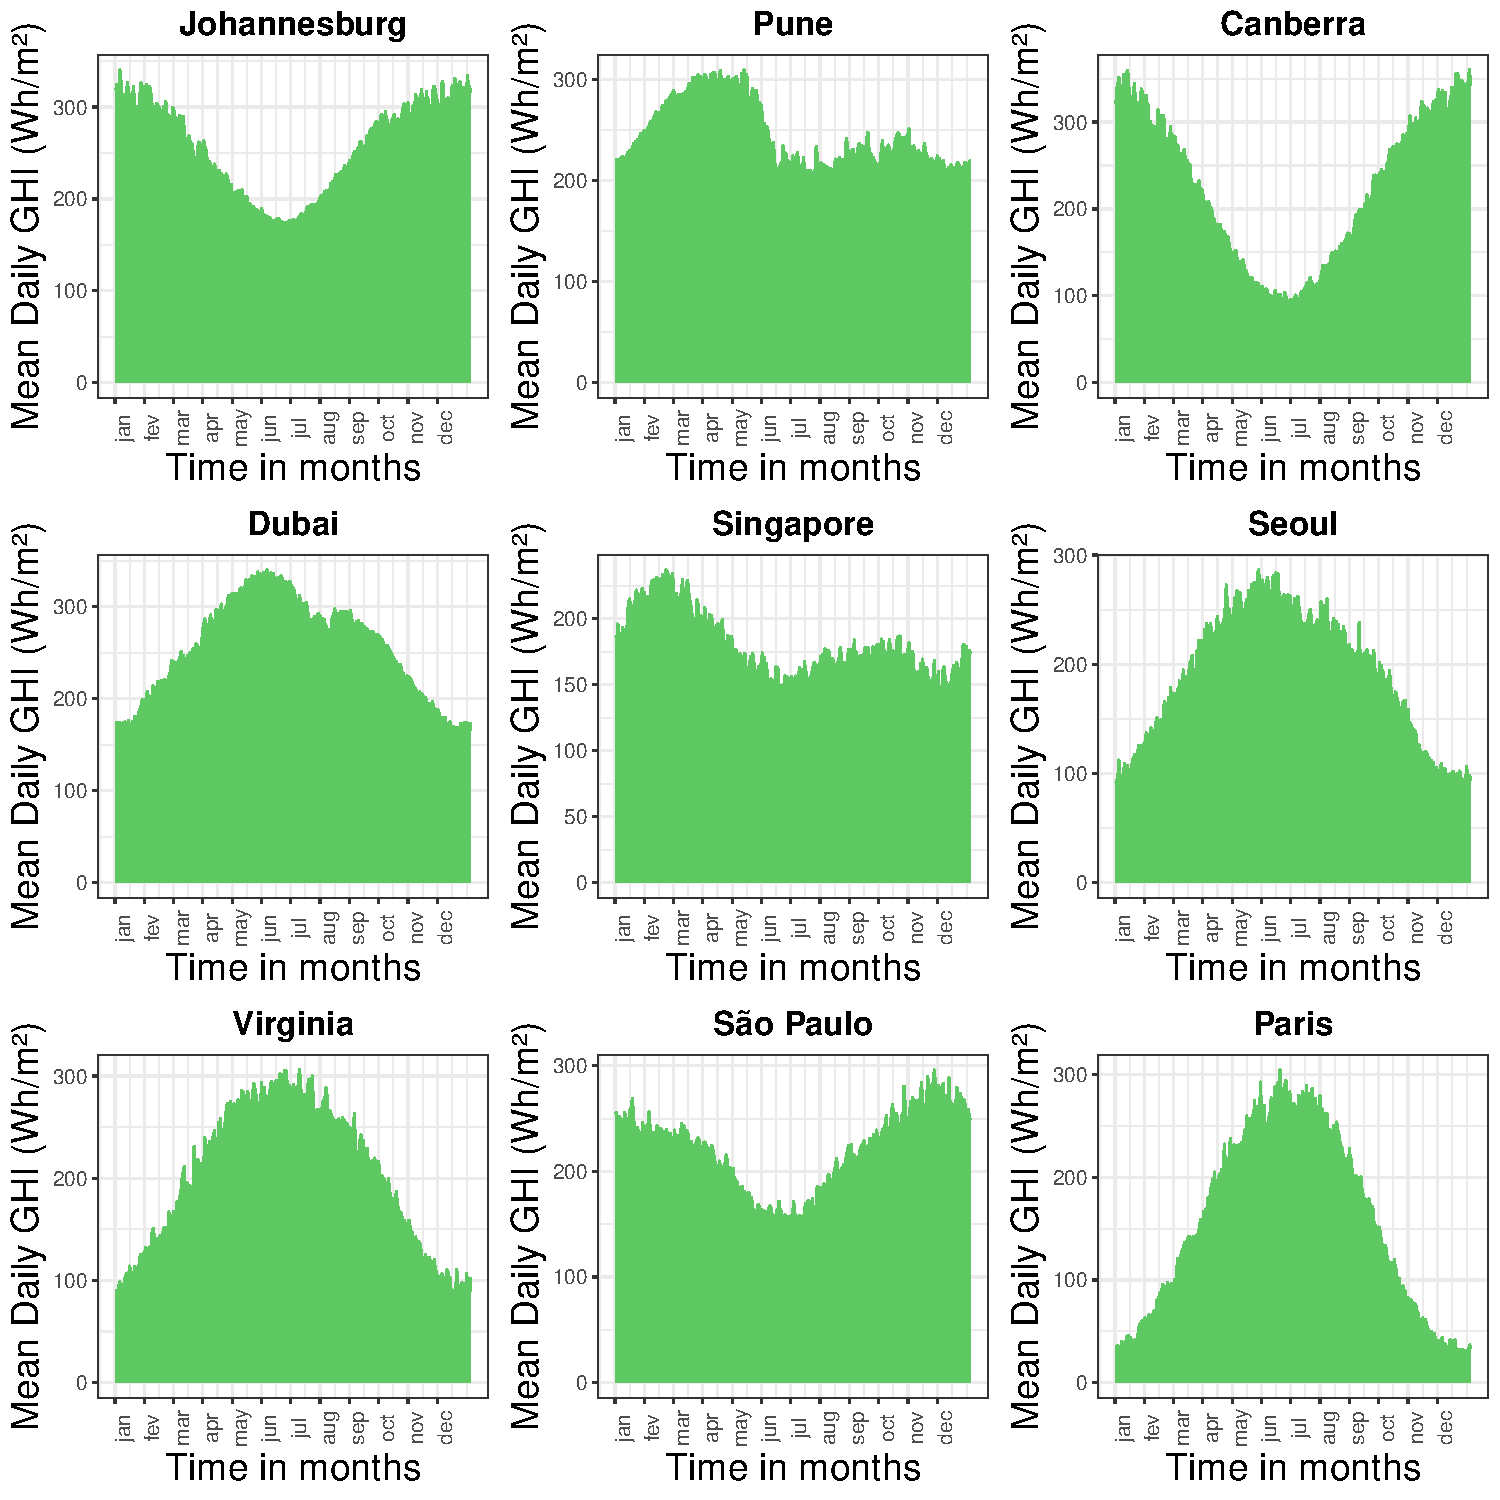
\epsfig{file = images/pv_daily_ghi_avg.pdf, width = .8\linewidth}}
   \caption{Average solar irradiation from 1980 to 2019 per location.}
  \label{fig:pv_ghi_avg}
\end{figure}

For the life-cycle \ch{CO2} emissions of the batteries and PVs, we used values from the National Laboratory of Renewable Energy (NREL) of the United States that performed an analysis with over 3000 published studies on the life-cycle of renewable infrastructures \cite{nrel_lifecycle_2021}: 43 $g\,\ch{CO2}\text{-}eq/kWh$ for the PVs and 33 $g\,\ch{CO2}\text{-}eq/kWh$ for the Lithium-Ion batteries.

\subsubsection{Results}

Table~\ref{tab:emissions_LCA} presents the \ch{CO2} emissions considering the whole life cycle, compared to considering only the one from manufacturing. As expected, the total \ch{CO2} emissions are higher (around 8\% increase) since the whole life cycle of the renewable infrastructure is now taken into account.

\begin{table}[!ht]
  
\caption{Total emissions for the different scenarios.}\label{tab:emissions_LCA} \centering

\begin{tabular}{|l|r|}
  \hline
  \textbf{Scenarios} & \textbf{Emissions ($\mathbf{t\,\ch{CO2}\text{-}eq}$)}   \\
  \hline  
    \ch{CO2} from manufacturing   & 34 559.03    \\  
  \hline
    \ch{CO2} from the whole life cycle       & 37 828.49    \\
  \hline


\end{tabular}
\end{table}


Finally, to better assess the impact of considering the emissions from the whole life cycle of the sizing process, we compare its results with those of the sizing process that only considers the emissions from the manufacturing phase---Figures~\ref{fig:pv_lca} and ~\ref{fig:bat_lca}.


\begin{figure}[H]
  \centering
  {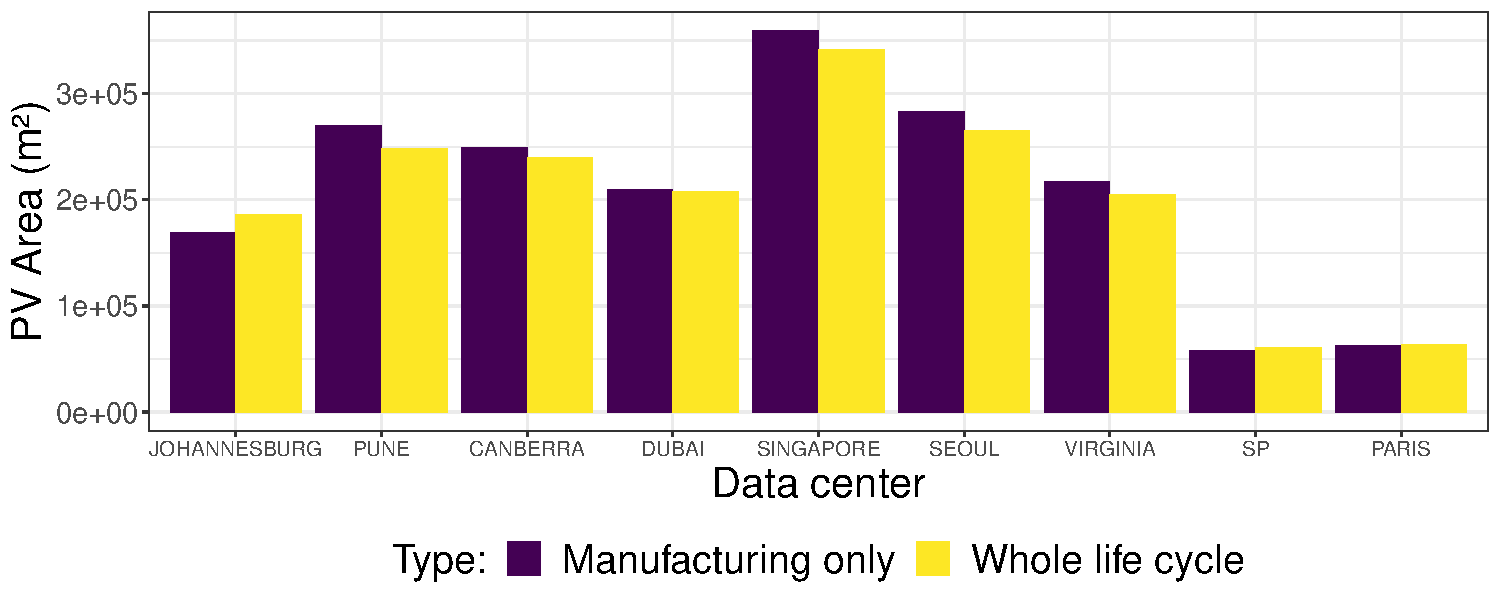
\epsfig{file = images/pv_sizing_after_lca.pdf, width = .8\textwidth}}
  \caption{PV Area sizing when considering the carbon footprint of manufacturing vs. the whole life cycle. }
  \label{fig:pv_lca}
\end{figure}


\begin{figure}[H]
  \centering
  {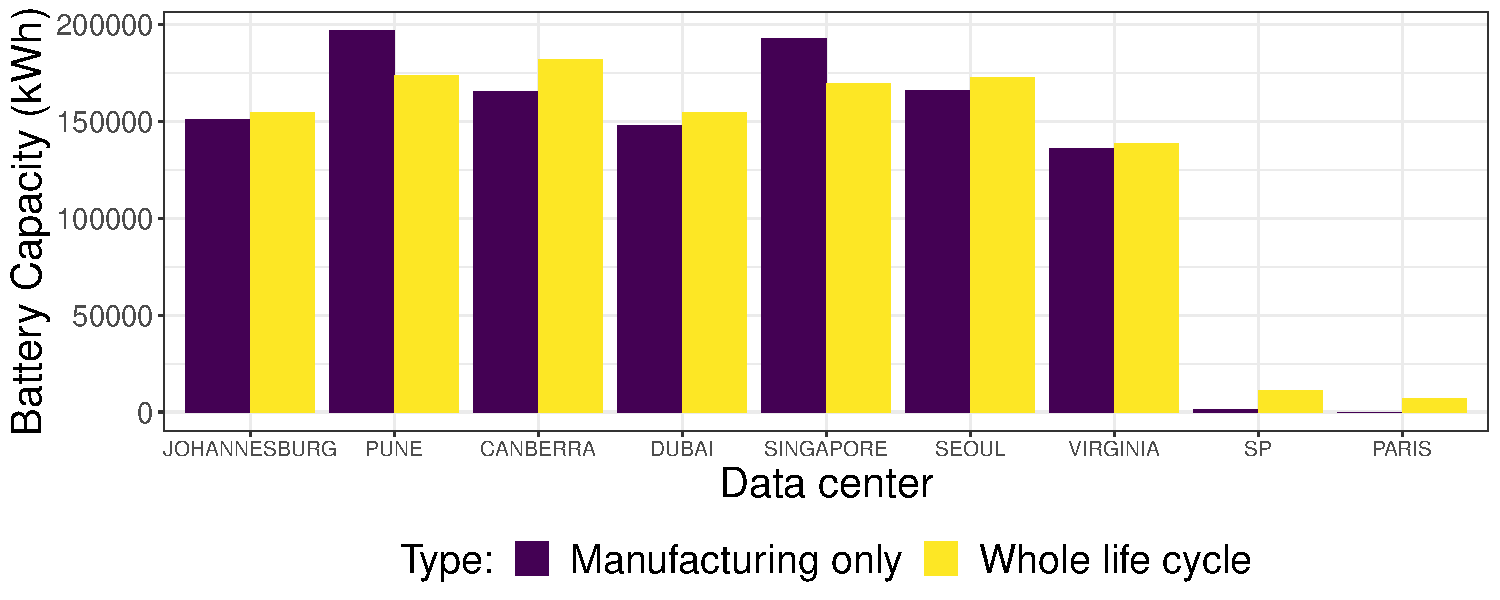
\epsfig{file = images/bat_sizing_after_lca.pdf, width = .8\textwidth}}
  \caption{Battery capacity sizing when considering the carbon footprint of manufacturing vs. the whole life cycle.  }
  \label{fig:bat_lca}
\end{figure}



\section{Including wind turbines to the renewable infrastructure}
\label{sec:add_wt}


In this section, we evaluate the impact on the carbon footprint of adding wind turbines (WT) as a power source to the on-site renewable infrastructure. Wind turbines may complement the photovoltaic power production to reduce the total emissions of the cloud federation operation, in particular during the night and seasons with lower solar irradiation, such as the winter. On the other hand, solar irradiation presents a lower variance than wind speed \cite{krakauer2017prediction_accuracy}.

\subsection{Updates in the model}
\label{sec:ex_model_wt}

We consider a new variable $WT^d$ representing how many wind turbines will be built at each DC location. The number of wind turbines (WT) is an integer number (we cannot produce 1.2 WT, for example). However, to avoid increasing the computational complexity of the LP by including integer variables, we made a relaxation in our modeling to allow the WT variable to be linear. 

The power production of the $WT^d$ wind turbines at the location of the data center $d$ at instant $k$ ($Pwt^d_{k}$) is modeled by Equation~\ref{eq:wt_power_prod}, where $V^d_k$ is the wind speed at location of the data center $d$ at instant $k$; $Vici$ is the \textit{cut in} wind speed, that is, the wind turbines start producing power when the wind speed is greater or equal to $Vici$; $Vco$ is the \textit{cut out} wind speed, that is, the wind turbines stop producing power when the wind speed is greater than $Vco$; $Pr$ is the rated power production in Watts of the wind turbine; and $Vr$ is the speed where the WT starts producing $Pr$ power. This model is based on \cite{HADDAD2021100505}.


\begin{equation} \label{eq:wt_power_prod}
Pwt^d_{k} = WT^d \times \left\{ 
  \begin{array}{ c l }
    0   & \quad \textrm{if } V^d_k \leq Vici \\
    Pr \times \frac{V^d_k - Vici}{Vr - Vici}  & \quad \textrm{if } Vici < V^d_k \leq Vr \\
    Pr  & \quad \textrm{if } Vr < V^d_k \leq Vco \\
    0  & \quad \textrm{if } Vco < V^d_k \\
  \end{array}
\right.
\end{equation}


Given that we are using additional renewable power infrastructure, it is also necessary to update the model of the renewable power production on DC $d$ at instant $k$. Equation~\eqref{eq:new_renewable_power} models that renewable power can originate from both PVs and WT.

\begin{equation} \label{eq:new_renewable_power}
    Pre^d_{k}= Ppv^d_{k} + Pwt^d_{k}
\end{equation}


To model the carbon footprint of the wind turbines, their whole life cycle also needs to be taken into account. Equation~\eqref{eq:fp_using_wt} models the footprint of using the WT at the location of the data center $d$ at instant $k$, where $wtCO2LC$ is the input that represents its emissions for the life cycle (in $g\,\ch{CO2}\text{-}eq/kWh$).

\begin{equation}\label{eq:fp_using_wt}
   FPwt^d_k =  wtCO2LC^d \times Pwt^d_{k}\times \Delta t
\end{equation}

Finally, the objective function also needs to be modified in order to include the carbon emissions from using WTs. Equation~\ref{eq:new_obj_co2_wt} models the new objective function.

\begin{equation} \label{eq:new_obj_co2_wt}
  \text{minimize }\sum_{k=0}^{K-1} \sum_{d=1}^D (FPgrid^d_k +  FPpv^d_k +  FPwt^d_k + FPbat^d_k) 
\end{equation}

\subsection{Experiments}

In order to analyze the impact of including wind turbines in the renewable infrastructure in terms of carbon footprint and dimensions of the solar panels and batteries, we perform the sizing and use the previous model---which considered only the PV and batteries---as a baseline.

\subsubsection{Settings}
\label{sec:settings_wt}

The cloud infrastructure, the workload, grid emissions, and the execution environment are the same as in Section~\ref{sec:settings_ccgrid}. The solar irradiation values, and emissions from PV panels and batteries are the same as Section~\ref{sec:ex_lca_pv}. For the \ch{CO2} emissions of the wind turbines, it is considered that they emit 13 $1g\,\ch{CO2}\text{-}eq/kWh$ taking into account its life cycle. The source for the values was the same as in Section~\ref{sec:ex_lca_pv}, the analysis from NREL that evaluated more than 3000 studies.

For the wind speed data, we used values from the ERA5 data source \cite{era5_wind_2022}---an average of the years 1980 to 2019. The data source contains values for the 100m v-component of wind (air horizontal speed towards the east) and the 100m u-component of wind (air horizontal speed towards the north)---both values are at 100 m of height. To transform these values into wind speed, we need to execute the following computation using Pitagora's theorem: $ w_s = \sqrt{ v^2 + u^2} $, where $w_s$ is the wind speed, $u$ the value of the u-component, and $v$ the value of the v-component.
\subsubsection{Results}
\label{sec:results_wt}

To evaluate the impact of including WT, we compare the sizing for using only PVs and batteries and using PV, batteries and WT. Table~\ref{tab:total_wind_and_pv_co2} presents the results in terms of total emissions. When also considering the wind as a renewable power source, we observe a reduction of approximately 34\% in comparison with the scenario where no WT is used and green energy is only produced by the PVs.

\begin{table}[h]  
  \caption{Total emissions ($t\,\ch{CO2}\text{-}eq$) for different scenario. }\label{tab:total_wind_and_pv_co2} \centering  
  \begin{tabular}{|l|r|}
  \hline    
  \textbf{Scenario} &   \textbf{Total emissions ($\mathbf{t\,\ch{CO2}\text{-}eq}$)} \\
  \hline    
  PV + Bat + WT + Grid  & 24 977.89 \\    
  \hline
  PV + Bat + Grid       & 37 828.49 \\    
  \hline
\end{tabular}  
\end{table}


Table~\ref{tab:results_wt} presents the number of WTs manufactured at each data center location. As said in Section \ref{sec:ex_model_wt}, we use a linear number for the wind turbines to avoid increasing the computational complexity of the problem. The decision-maker could decide whether to round the value up or down based on its budget constraints.

\begin{table}[h]
  \caption{Computed number of WT for each location.}\label{tab:results_wt} \centering
  \begin{tabular}{|l|r|}
  \hline
    
  \textbf{Location} &   \textbf{Number of WT} \\
  \hline
  Johannesburg & 58.11   \\
  \hline
  Pune  & 25.77 \\
  \hline
  Canberra  & 66.56 \\
  \hline
  Dubai   &  79.09  \\
  \hline
  Singapore & 36.93  \\
  \hline     
  Seoul    & 109.56  \\
  \hline
  Virginia   & 39.16 \\
  \hline
  São Paulo   & 86.53 \\
  \hline 
  Paris    &   22.15 \\
  \hline
  
\end{tabular}  
\end{table}

The Capacity Factor metric can be used to better analyze the potential of a location to generate renewable power. This metric measures a ratio of the real energy produced by the device in comparison to its maximum energy output~\cite{NREL_2012_capacityfactor}. In our experiments, we used the rated power of 150 W for a 1 square meter solar panel, and we used climate conditions from 1980 to 2019 to estimate the Capacity Factor. Table~\ref{tab:capacity_factor} presents the results for both the PV and wind turbines.

\begin{table}[H]
  
  \caption{Capacity Factor (in \%) for solar panels and wind turbines at each location.}\label{tab:capacity_factor} \centering
  
  \begin{tabular}{|l|r|r|}
  \hline    
  \textbf{Location} &   \textbf{PV} & \textbf{WT}  \\
  \hline
  Johannesburg & 25.55 & 12.96  \\
  \hline
  Pune        &  24.26   & 10.04    \\
  \hline
  Canberra    & 22.08    & 12.97  \\
  \hline
  Dubai      & 25.28      & 13.98   \\
  \hline
  Singapore & 17.68    & 8.58   \\
  \hline     
  Seoul      & 18.81   &  9.41   \\
  \hline
  Virginia   & 19.83   &  14.68 \\
  \hline
  São Paulo  & 21.74   &  10.06    \\
  \hline 
  Paris      & 15.37   &  23.51   \\
  \hline  

\end{tabular}
\end{table}


Finally, to assess the impact of including the WT regarding the sizing of both PV and batteries, we present in Figure~\ref{fig:wind_pv} and Figure~\ref{fig:wind_bat}  the dimensioning for both equipment considering and not considering manufacturing WT. It is possible to observe that the inclusion of wind turbines has a significant reduction in the total solar panel area, and for some locations---such as São Paulo and Paris---the optimal is to use only wind turbines. The batteries are also reduced, given that the wind can blow at night as well, so no extra energy needs to be charged in the batteries from the solar panels to be used for night computations.

\begin{figure}[H]
  \centering
  {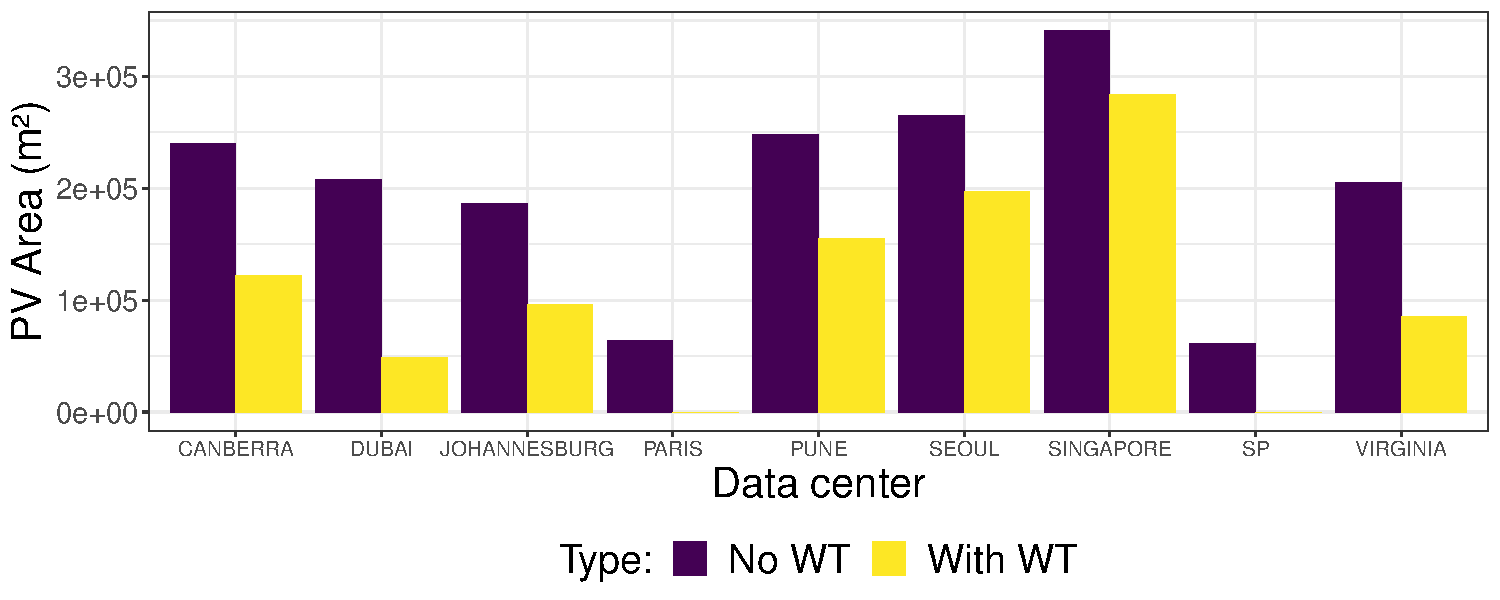
\epsfig{file = images/pv_sizing_after_wt.pdf, width = .8\textwidth}}
  \caption{PV Area sizing when the WT are and are not included. }
  \label{fig:wind_pv}
\end{figure}


\begin{figure}[H]
  \centering
  {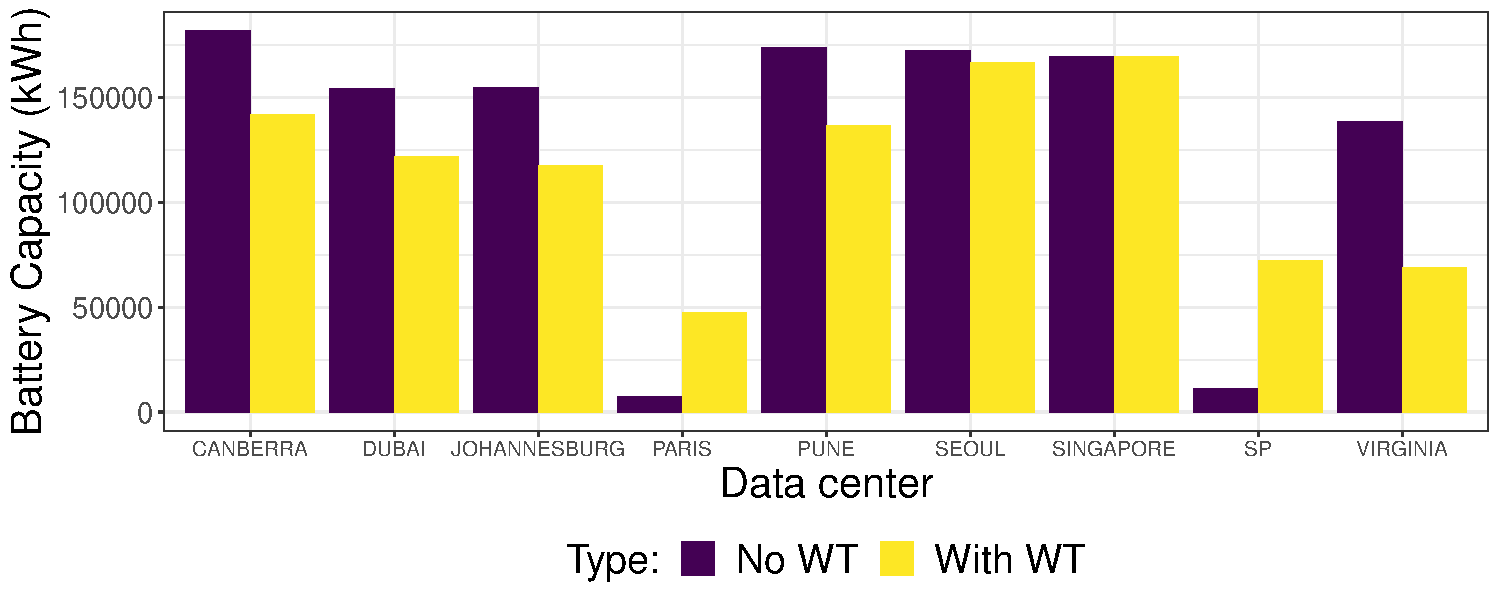
\epsfig{file = images/bat_sizing_after_wt.pdf, width = .8\textwidth}}
  \caption{Battery capacity sizing when the WT are and are not included. }
  \label{fig:wind_bat}

\end{figure}


\section{Sensibility of the LP to  uncertainties}
\label{sec:sensitivity}

To assess the sensibility of the linear program to the inputs, we evaluate it considering different scenarios in terms of solar irradiation, wind speed, and grid emissions data. The renewable sources are intermittent by nature, and this variation can impact the sizing process, resulting in an over- or under-sizing of the renewable infrastructure.


In order to illustrate the intermittency of both wind speed and solar irradiation, we present in Figure~\ref{fig:pv_boxplots} boxplots of the total energy one solar panel produced per year during the years 1980 to 2019, and in Figure~\ref{fig:wt_boxplots} for a single wind turbine. Those figures illustrate the intermittency of renewable power production over the years, and one may also observe the potential for using one source or another: for example, Paris has the lowest solar power production considering one solar panel, and on the other hand, it has the highest wind power production. 

\begin{figure}[H]
  \centering
  {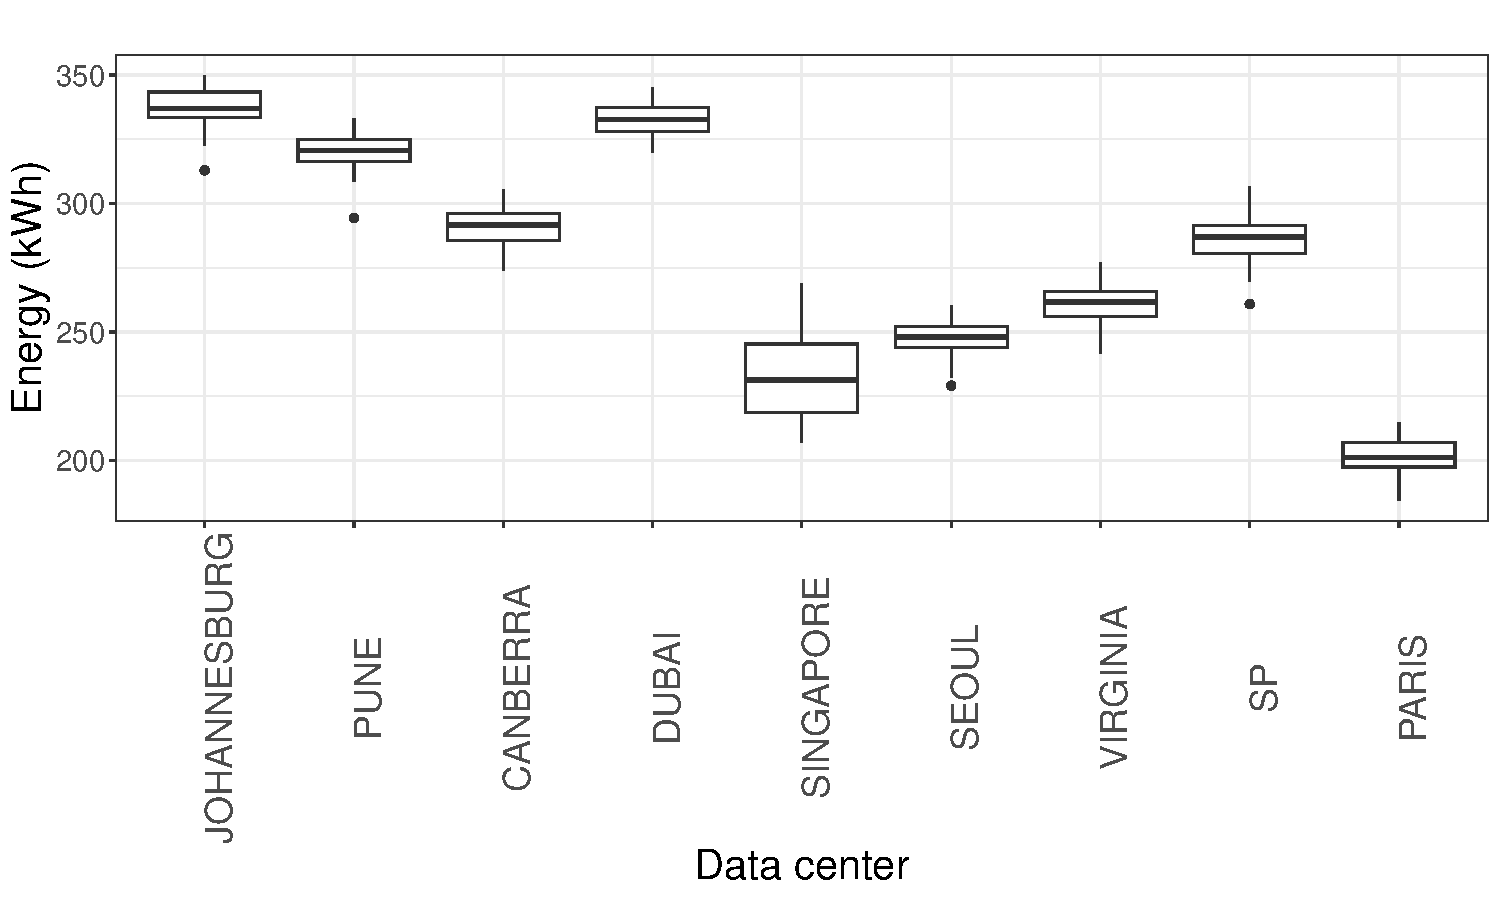
\epsfig{file = images/energy_pv.pdf, width = \textwidth}}
  \caption{Different energy production for 1 PV panel at each location for the years 1980 to 2019.}
  \label{fig:pv_boxplots}
\end{figure}


\begin{figure}[H]
  \centering
  {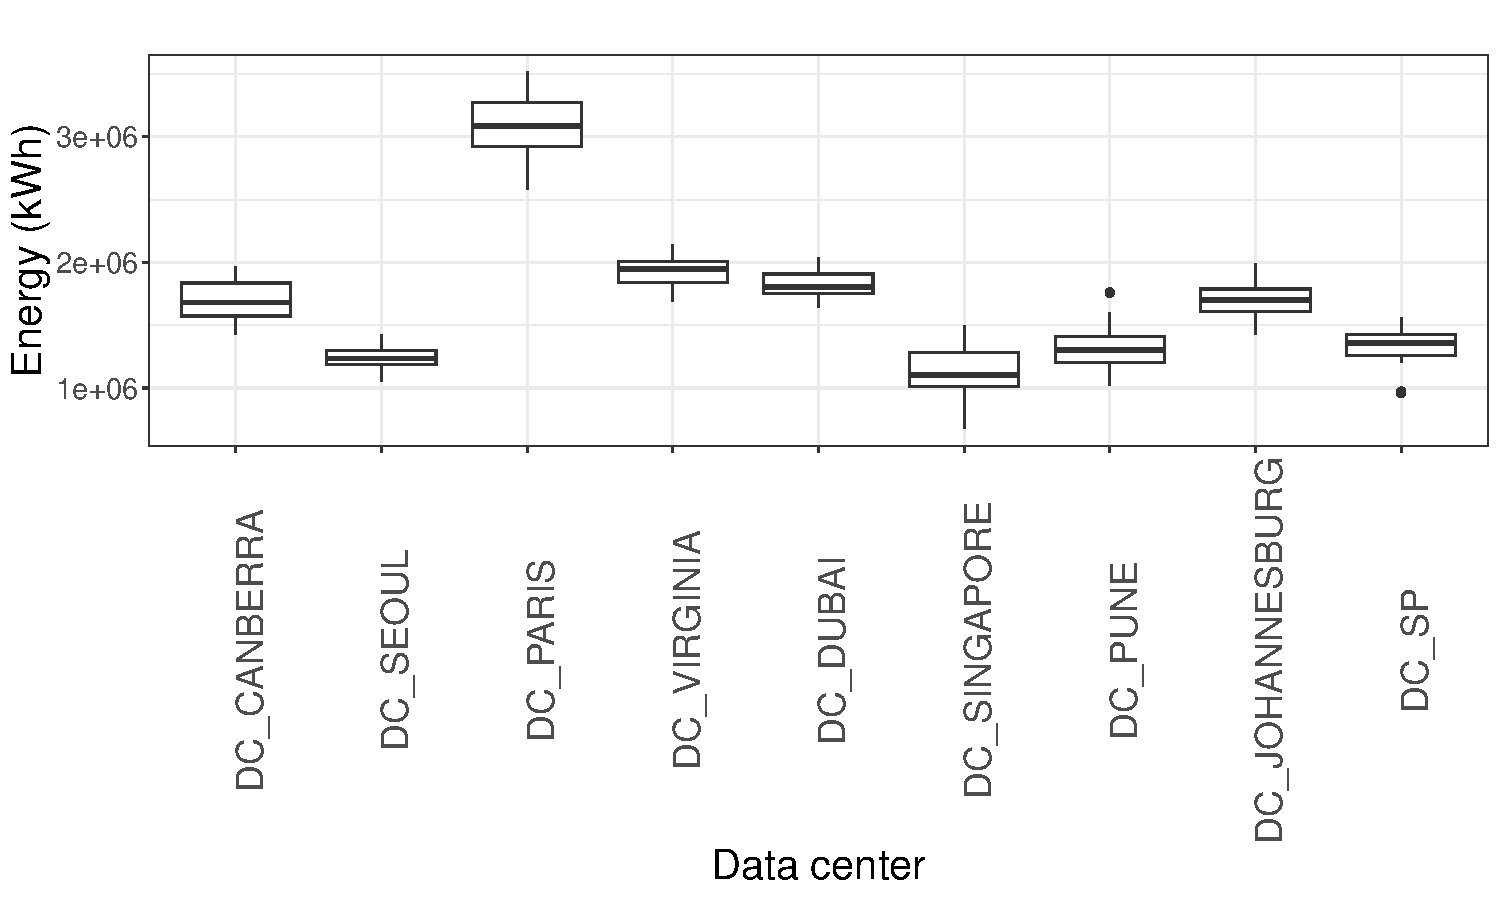
\epsfig{file = images/energy_wt.pdf, width = \textwidth}}
  \caption{Different energy production for 1 wind turbine at each location for the years 1980 to 2019.}
  \label{fig:wt_boxplots}
\end{figure}



Given the presence of low-carbon-intensive power sources in some countries, the emissions of the local electricity grid are not static all year. For example, regions with access to solar energy have a lower grid footprint during the day. Some countries provide access to fine-grain information about their electricity mix in real-time or historical data in the form of time series. However, obtaining data for all the locations is not an easy process: not all the locations provide this information, or they provide different time granularity (day, hour, month), historical data with different durations (for example, only the last six months), or only real-time values. For modeling the variation in grid emissions, it is necessary to update the model, and in the next section, we present the modifications.

\subsection{Updates in the model}

\subsubsection{Intermittency of renewable sources}

Regarding the intermittency of solar irradiation and wind speed, there are no necessary modifications to be made in the modeling itself, as the impact is generated by the input data that will be used for the sizing process.
\subsubsection{Fine-grain values of grid emission data (hour by hour)}

To model the change in the electricity grid emissions over time, we need to modify the input $gridCO2^d$ to be a time series. For locations where data is not available hourly, pre-processing of the data is needed. For example, if the region only provides daily data, one can assume that for the 24 hours of the day, the value of grid emissions will be the same. Equation~\eqref{eq:fpgrid_timeseries} presents the modification where $gridCO2^d_k$ is the new input for the grid emissions with one value for each time slot $k$ at the location of the data center $d$.

\begin{equation} \label{eq:fpgrid_timeseries}
FPgrid_k^d = Pgrid_k^d\times \Delta t \times gridCO2^d_k
\end{equation}

\subsection{Experiments}

To assess the sensitivity of the model to the inputs of climate conditions and grid emissions, we conducted a series of experiments. For the climate conditions, we evaluate if using simple forecasts provides precise results and what the impact is on the carbon footprint considering the future operation---10 years, and the baseline is the optimal scenario where the climate conditions are known in advance. For the grid emissions, we evaluate the impact on the carbon footprint by using the fine-grain information---hourly---and the average year value.


\subsubsection{Settings}


For both scenarios, the cloud infrastructure, the workload, and the execution environment are the same as in Section~\ref{sec:settings_ccgrid}.

\paragraph{Intermittency of renewable sources}

To evaluate the sensibility of the sizing process considering the uncertainty of the production of renewable sources , we compare---in terms of \ch{CO2} emissions---the operation of the cloud federation using the optimal renewable infrastructure (where all the climate conditions are known in advance) with a renewable infrastructure dimensioned using simple forecasting techniques (average and median from the past). The scenarios are described as follows. First, we collected average and median solar irradiation and wind speed values per time slot from 1980 to 2009 to create inputs for the sizing process. Second, we executed the sizing process using the climate conditions generated in the previous step. Then, the cloud was operated for ten years (2010 to 2019) using the dimensions (PV area, number of wind turbines, and capacity of batteries) computed by the sizing process step, but with the climate conditions of each respective year. Finally, the results in terms of \ch{CO2} emissions were compared to the optimal renewable infrastructure from 2010 to 2019.

We also evaluate the adoption of PV only and WT only in the sizing, to assess which impacts the sizing process more. The evaluation follows the same steps described in the previous paragraph.

The data for the solar irradiation was collected from the MERRA-2 project~\cite{GELARO2017MERRA2}, and for the wind speed from the ERA5 data-source \cite{era5_wind_2022}.

\paragraph{Fine-grain values of grid emission data (hour by hour)}

In order to evaluate the impact of using a fixed value for the grid emissions (an average of the year)  or a fine grain value (hourly time series), we perform the sizing with these two scenarios and compare them in terms of \ch{CO2} emissions and dimensions of the renewable infrastructure for the years 2018, 2019, 2020 and 2021.

For the scenario of hourly grid emissions, we used data sources provided by Electricity Map. For the locations: Pune, Canberra, Seoul, Virginia, São Paulo, and Paris, the data source provides \ch{CO2} intensity of the grid hour by hour for the duration of 1 year. For the Johannesburg and Singapore regions, the information on \ch{CO2} emissions was in the granularity of months. Therefore, we generated a time series with a total duration of one year and the same value of \ch{CO2} per hour for each corresponding month. For Dubai, we only found data for the year's average grid \ch{CO2} emissions, and we generated a time series in which the grid emissions are fixed for every hour of the year.


Table~\ref{tab:grid_emissions_hist} presents the sources of the data, the time span, and the granularity for the grid emissions of each data center location, and Table~\ref{tab:grid_emissions_avg_year} presents the average \ch{CO2} emissions of the year for these data sources---the value used is the average of the time series of each location for the evaluated years.

\begin{table}[h]  
\caption{Comparison of local electricity grid  information. }\label{tab:grid_emissions_hist} \centering  
  \begin{tabular}{|l|r|r|r|}
    \hline
    
  \textbf{Location} &   \textbf{Granularity} & \textbf{Span} & \textbf{Source} \\
  \hline
  Johannesburg & month & year & ElectricityMaps  \\
  \hline
  Pune  & hour & year & ElectricityMaps  \\
  \hline
  Canberra  & hour &  year & ElectricityMaps \\
  \hline
  Dubai    & year & year & 1.5°C national pathway explorer  \\                       
  \hline
  Singapore & month & year & ElectricityMaps \\
  \hline     
  Seoul     & hour & year & ElectricityMaps \\
  \hline
  Virginia  &  hour & year & ElectricityMaps \\
  \hline
  São Paulo & hour & year  & ElectricityMaps \\
  \hline 
  Paris     & hour & year  & ElectricityMaps  \\
  \hline
\end{tabular}  
\end{table}


\begin{table}[h]
  \caption{Average emissions (in $g\,\ch{CO2}\text{-}eq/kWh$) from using the regular grid at the different years.}\label{tab:grid_emissions_avg_year} \centering
  \begin{tabular}{|l|r|r|r|r|}    
  \hline   
  \textbf{Location} &  \textbf{2021} & \textbf{2020} & \textbf{2019} & \textbf{2018}\\
  \hline
  Johannesburg & 700.66 & 700.66 & 700.66 & 700.66  \\
  \hline
  Pune & 728.15 & 724.04 & 726.43 & 723.83     \\
  \hline
  Canberra & 655.36 & 692.23 & 712.43 & 728.21\\
  \hline
  Dubai & 530.00  & 530.00 & 530.00 & 530.00     \\
  \hline
  Singapore & 491.01 & 491.01 & 491.01 & 491.01 \\
  \hline     
  Seoul & 490.60 & 490.15 & 490.73 & 490.90     \\
  \hline
  Virginia  & 435.25 & 415.14 & 447.98 & 453.40 \\
  \hline
  São Paulo &  172.54 &  103.47 & 108.95 &  105.21 \\
  \hline 
  Paris &  63.48  & 62.99 & 61.62   & 60.00   \\
  \hline

\end{tabular}  
\end{table}


To illustrate the variations of the grid emission over time, we present two scenarios to the reader: one with a significant presence of renewables in the local electricity grid (São Paulo) and another with a low presence (Seoul). It will be possible to observe the differences between day and night, seasons, and years.


Figure~\ref{fig:co2_sp} illustrates the local electricity grid emissions over time for São Paulo, and each subplot represents one quarter of the year (3 months). The differences between day and night might be justified by using solar energy, and the differences between seasons. However, it is also possible to observe a difference among the years---2021 is the year with the highest grid carbon footprint. The higher emissions of the year 2021 are justified by the hydric crisis that occurred during that period---the greatest of the previous 91 years---and since a large share of São Paulo's electricity demand is supplied by hydroelectric power, coal power plants were used to meet the power demand~\cite{CNN2021_crisehidrica}.

\begin{figure}[H]
  \centering
  {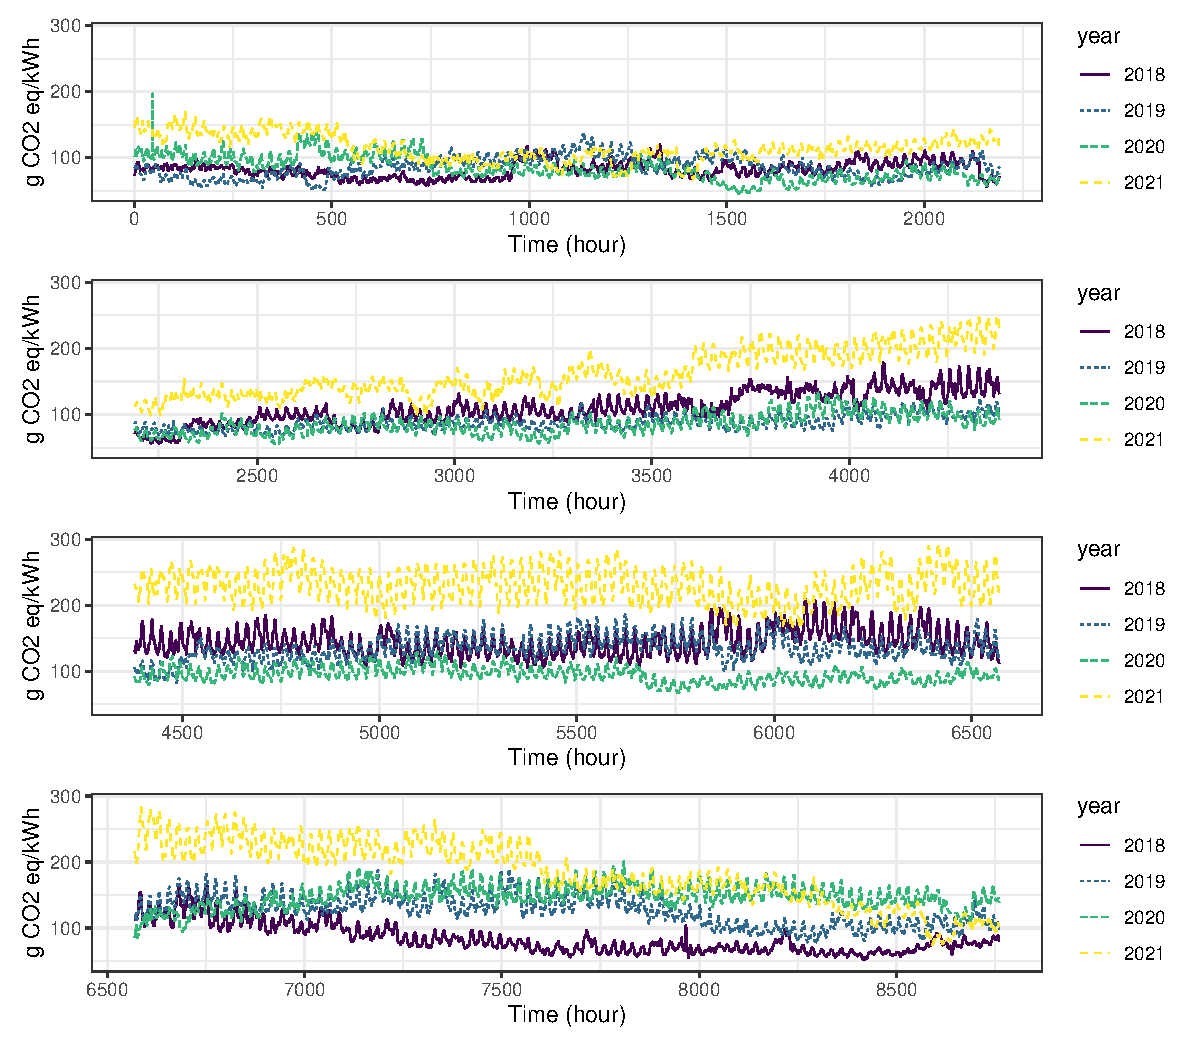
\epsfig{file = images/co2_emissions_sp.pdf, width = \textwidth}}
  \caption{São Paulo's hour by hour grid emissions for the years 2018, 2019, 2020 and 2021.}
  \label{fig:co2_sp}
\end{figure}

The scenario of Seoul---illustrated in Figure~\ref{fig:co2_seoul}---represents a location with a low presence of renewables: most of the electricity demand is supplied by carbon-intensive sources such as coal and gas. The usage of PV panels can justify the small variation between the hours, as when the sun starts shining, they produce power and the emissions are reduced.

\begin{figure}[H]
  \centering
  {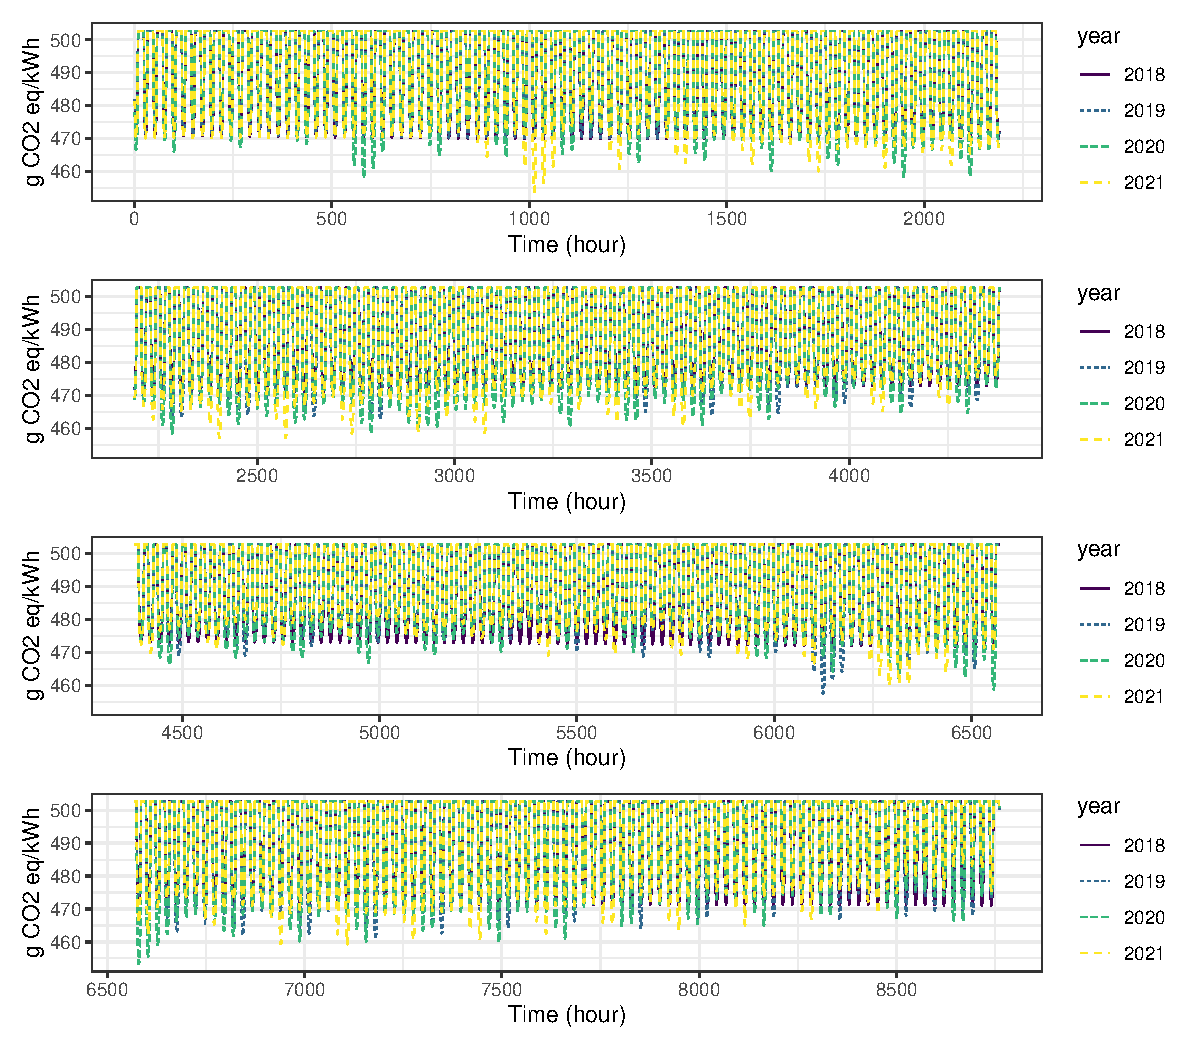
\epsfig{file = images/co2_emissions_seoul.pdf, width = \textwidth}}
  \caption{Seoul's hour by hour grid emissions for the years 2018, 2019, 2020 and 2021.}
  \label{fig:co2_seoul}
\end{figure}




\subsubsection{Results}

\paragraph{Intermittency of renewable sources}

Table~\ref{tab:co2_10y} presents the results in terms of \ch{CO2} emissions for the renewable infrastructure that included both PV panels and wind turbines, and in Table~\ref{tab:co2_10y_pv_only} only PV panels are considered.



 \begin{table}[H]   
  \caption{Emissions (in kt \ch{CO2}-eq) for the different scenarios---renewable infra only have PV panels and batteries.} \centering

   \label{tab:co2_10y_pv_only}
  
      \begin{tabular}{|l|r|r|}        
        \hline
        \textbf{Sizing Scenario} &  \textbf{Emissions } & \textbf{Diff. to baseline (\%) } \\
       \hline        
        Optimal sizing 2010-2019       &       408.767 &  -       \\
        \hline     
        Average irradiation 1980-2009  &       414.956 &  1.49    \\
        \hline
        Median irradiation  1980-2009  &       422.928 &  3.35   \\
        \hline        
      \end{tabular}
      
    \end{table}


    
 \begin{table}[H]   
  \caption{Emissions (in kt \ch{CO2}-eq) for the different scenarios---renewable infra only have wind turbines and batteries.} \centering

   \label{tab:co2_10y_wt_only}
  
      \begin{tabular}{|l|r|r|}        
        \hline
        \textbf{Sizing Scenario} &  \textbf{Emissions } & \textbf{Diff. to baseline (\%) } \\
        
        \hline
        Optimal sizing 2010 - 2019       &       710.351 &  -        \\
        \hline     
        Average wind speed 1980 - 2009  &       777.957 &  9.5      \\
        \hline 
        Median wind speed  1980 - 2009  &       770.891 &  8.5      \\
        \hline        
      \end{tabular}      
    \end{table}

       
\begin{table}[H]
  \caption{Emissions (in kt \ch{CO2}-eq) for the different scenarios---renewable infra has PV panels, wind turbines and batteries.} \centering
    \label{tab:co2_10y}
      \begin{tabular}{|l|r|r|}        
        \hline        
        \textbf{Sizing Scenario} &  \textbf{Emissions } & \textbf{Diff. to baseline (\%) } \\
        \hline        
        Optimal sizing 2010-2019  &       301.931 & - \\
        \hline     
        Average irrad. and wind speed  1980-2009  &      342.584 &  11.9 \\
        \hline
        Median irrad. and wind speed  1980-2009  &      340.784 &   11.4 \\
        \hline        
      \end{tabular}      
    \end{table}

    
\paragraph{Fine-grain values of grid emission data (hourly)}

Table~\ref{tab:co2_grid_granularities_years} presents the increase in \ch{CO2} emissions (relative value in percent) of not having access to the fine-grain value of \ch{CO2} emissions (as hourly values).


\begin{table}[H]

  \caption{Difference in total emissions (\%) between the scenario where the sizing used the grid year's average value in comparison to using hourly information.}\label{tab:co2_grid_granularities_years} \centering

  \begin{tabular}{|l|r|r}
    \hline
    
  \textbf{Year} &   \textbf{Difference (\%) in \ch{CO2} emissions} \\
  \hline
  2018 &   0.34 \\
  \hline
  2019 &   0.59 \\
  \hline
  2020 &   0.18 \\
  \hline
  2021 &   0.74 \\
  \hline

\end{tabular}  
\end{table}


\section{Scheduling flexibility to reduce \ch{CO2} emissions}

One of the challenges in the sizing process is that once built, the dimensions of the renewable infrastructure cannot be reduced---this would imply destroying them, resulting in an environmental impact and a waste of money. The intermittency of renewable sources could generate this oversizing of the infrastructure. In this section, we evaluate how workload scheduling may mitigate the effects of a bad-sizing process and, in particular, what the gains are in reducing carbon emissions if we delay the execution of the workload to handle renewable power fluctuations.

\label{sec:flexibility}

\subsection{Updates in the model}

Suppose that we have the flexibility to delay $\alpha$ percent of the workload up to $\beta$ time slots. We need two new variables to model this new feature. Let $alloc^d_k$ represent the required number of CPU cores  to execute the workload allocated to the data center $d$ at the time slot $k$ and $delay_{k,i}^d$ be the required number of CPU cores to execute the workload of the data center $d$ that can be delayed from time slot $k$ up to $\beta$ time slots ($i$ is the index of the list of size $\beta$ for the delayed workload). 

This feature also requires new restrictions. Equation~\eqref{eq:alpha} models the flexibility of allowing $\alpha$ percent of the workload to be delayed, where $W_k$ is the input that represents the total CPU core demand to execute the workload at time slot k.


\begin{equation} \label{eq:alpha}
   \sum_{d=1}^D  \sum_{i=1}^{\beta} delay_{k,i}^d \leq  \alpha   \times W_k
\end{equation}


Equation~\eqref{eq:beta} models the flexibility to delay the workload up to the next $\beta$ time slots and ensure that all the workload will be executed:


\begin{equation} \label{eq:beta}
  \sum_{d=1}^D    (alloc_k^d +    \sum_{i=1}^{\beta} delay_{k,i}^d) = W_k  
\end{equation}


The allocated workload at a time slot k, and the delayed workloads from the previous k - $\beta$ time slots need to respect the data center servers's CPU core capacity. Equation ~\eqref{eq:beta_capacity} models this restriction.
     
\begin{equation} \label{eq:beta_capacity}
\sum_{d=1}^D    (alloc_k^d  +    \sum_{i=k-\beta}^{k-1} delay_{  i ,  k-i  }^d)  \leq C_d 
\end{equation}

\subsection{Experiments}

To assess the reductions in carbon footprint we can achieve by delaying the workload, we perform a series of experiments with different combinations for the values of $\alpha$---how much of the workload it is possible to delay---and $beta$---how long it is possible to delay the workload---and compare them with the scenario where it is not possible to delay the workload.

\subsubsection{Settings}

The cloud infrastructure, the workload, grid emissions, and the execution environment are the same as in Section~\ref{sec:settings_ccgrid}. In order to evaluate only the impact of the flexibility of the scheduling on reducing carbon emissions, all the other parameters are fixed: workload, solar irradiation (average from 1980 to 2019), wind speed (average from 1989 to 2019), area of PV panels and the capacity of the batteries, number of wind turbines, power consumption of servers and network devices, and so on. We present an evaluation for delaying 10\% up to 50\% of the workload---$\alpha$ values of 0.1, 0.2, 0.3, 0.4, and 0.5---for the period of one hour up to one week---$\beta$ values of 1 h, 12 h, 24 h, 48 h, 96 h, 120 h, 144 h and 168 h.
\subsubsection{Results}

The results of the experiments in terms of reduction of \ch{CO2} emissions are presented in Table~\ref{tab:flex_scheduling}.


\begin{table}[h]
\caption{Reductions in total carbon emissions ( \% ) in comparison to the scenario where it is not possible to delay the workload. The $\alpha$ values represent how much of the workload can be delayed (in \%) and the $\beta$ values how long the workload can be delayed (in hours). }\centering
\label{tab:flex_scheduling}
\begin{tabular}{|l|r|r|r|r|r|r|r|r|r|}
\hline
\backslashbox{$\alpha$}{$\beta$} &   \textcolor{black}{\textbf{ 1}} &  \textcolor{black}{\textbf{ 12 }} &  \textcolor{black}{\textbf{ 24 }} &  \textcolor{black}{\textbf{ 48 }}  &   \textcolor{black}{\textbf{ 72 }} &   \textcolor{black}{\textbf{ 96 }} &   \textcolor{black}{\textbf{ 120  }} &   \textcolor{black}{\textbf{ 144 }} &   \textcolor{black}{\textbf{ 168 }} \\ 
     \hline
 \textcolor{black}{ \textbf{10}}   &  0.46 &  2.59 &  3.14 &  3.48 &  3.66 &  3.76 &  3.81 &  3.85 &  3.85 \\ 
\hline
 \textcolor{black}{ \textbf{20}}   &  0.84 &  3.4 &  3.85 &  4.11 &  4.21 &  4.21 &  4.21 &  4.22 &  4.22 \\ 
\hline
 \textcolor{black}{ \textbf{30}}   &  1.15 &  3.71 &  4.07 &  4.25 &  4.25 &  4.26 &  4.26 &  4.27 &  4.27 \\ 
\hline
 \textcolor{black}{ \textbf{40}}   &  1.42 &  3.89 &  4.15 &  4.25 &  4.26 &  4.27 &  4.28 &  4.28 &  4.29 \\ 
\hline
 \textcolor{black}{ \textbf{50}}   &  1.65 &  4.01 &  4.22 &  4.26 &  4.27 &  4.28 &  4.29 &  4.3 &  4.3 \\ 
\hline
\end{tabular}
\end{table}


\section{ Monetary costs of reducing the carbon emissions}
\label{sec:costs}

In the previous sections, we showed the results only in terms of the environmental impact of the cloud operation, now we present the results in terms of the monetary costs (in dollars) of operating the cloud platform and how much it would cost for the DC operator to reduce their environmental impact. This is also an important aspect, as the decision-makers want their business to be lucrative.

\subsection{Updates in the model}

To perform this new analysis, we need to make some modifications to our modeling. The first modification regards buying electricity from the regular grid, and it is modeled by Equation~\eqref{eq:pricegrid}, where $costGrid^d_k$ is an input that represents the costs of buying electricity at each location (in dollars per kWh) at time slot $k$.

\begin{equation} \label{eq:pricegrid}
 PriceGrid^d_k = Pgrid^d_k \times costGrid^d_k
\end{equation}

To measure the price of electricity from renewable sources, we can use the metric Levelized Cost of Energy (LCOE) \cite{nrel_economic_wt_1995}. This metric compares the total costs of manufacturing and operating the electricity infrastructure (for example, the PV panel) with the total energy it can deliver in its lifetime, and the metric is in the form of costs per unit of electricity generated---\$ per kWh.

Similar to the \ch{CO2} emissions of renewable sources, the price will also differ per location, as the total amount of irradiation and wind speed differ.

Equation~\eqref{eq:pricepv} models the costs of consuming energy from the solar panels, where $PVLCOE^d$ represents the specific LCOE at the location of the data center $d$ (in dollars per kWh).

\begin{equation} \label{eq:pricepv}
  PricePV^d_k = PPV^d_k \times PVLCOE^d
\end{equation}


For the wind turbines, we also use the LCOE to compute its price, and Equation~\eqref{eq:pricewt} models the costs of using energy from the WT, where $WTLCOE^d$ represents the specific LCOE at the location of the data center $d$ (in dollars per kWh).

\begin{equation} \label{eq:pricewt}
  PriceWT^d_k = PWT^d_k \times WTLCOE^d
\end{equation}

For the batteries, the metric Levelized Cost of Storage (LCOS) is similar to the LCOE, and it represents the cost per unit of energy discharged (dollars per kWh or MWh) that takes into account its whole life cycle: calendar and cycle life, Max Depth of Discharge limitations, and costs from operation and maintenance \cite{battery_lcos_2022}.  Equation~\eqref{eq:pricebat} models the costs of the energy used from the batteries using its LCOS as input ($BatLCOS$ in dollars per kWh of electricity discharged). To avoid oversizing the batteries, the restriction of Equation~\eqref{eq:b_initial_level} that makes the battery start empty at the beginning of the day is also used in this scenario.

\begin{equation} \label{eq:pricebat}
   PriceBat^d_k = Pdch^d_k \times BatLCOS
\end{equation}


We can also modify our objective function to minimize the price of operating the cloud platform instead of its environmental impact, and Equation~\eqref{eq:objective_price} models this new objective.
  
\begin{equation} \label{eq:objective_price}
\text{minimize }\sum_{k=0}^{K-1} \sum_{d=1}^D PriceGrid^d_k  + PriceBat^d_k + PricePV^d+ PriceWT^d_k
\end{equation}


\subsection{Experiments}

To analyze the monetary costs of operating the cloud federation, we present results in terms of price (millions of dollars) and carbon footprint (tons of \ch{CO2}-eq) for a series of experiments with both the objective of minimizing the monetary costs and the carbon emissions. Additionally, the reader is presented with a comparison of the dimensions of renewable infrastructure between the solutions of minimal monetary costs and minimal carbon footprint.

\subsubsection{Settings}

The cloud infrastructure, the workload, and the execution environment are the same as in Section~\ref{sec:settings_ccgrid}. In this scenario, since the objective is to minimize costs, the carbon footprint from the grid and renewable infrastructure is not considered for the experiments.

For the price of solar panel electricity, we use the tool ``Comparative Photovoltaic Levelized Cost of Energy Calculator'' from the National Renewable Energy Laboratory of the USA \cite{pv_lcoe_calc}---version 2.0.0 of August 2021. This tool provides a detailed cost model for many parts of the PV panel, with adequate default values. For reproducibility purposes, Table~\ref{tab:parameters_pv_LCOE} lists the values of the parameters used, and the only differences between the default values were for the parameters Service life, Performance Efficiency, and the Energy yield (that depends on the location where the PV module is installed). For the latter, the following values were considered:   1934.03 for Canberra;  1648.08 for Seoul; 1346.32 for Paris; 1737.38 for Virginia; 2215.17 for Dubai; 1549.23 for Singapore; 2125.62 for Pune;  2238.52 for Johannesburg; and 1904.66 for São Paulo.
\begin{table}[h]
  
  \caption{Parameters used in the LCOE PV calculator.}\label{tab:parameters_pv_LCOE} \centering

  \begin{tabular}{|l|r|}
    \hline    
    \textbf{Parameter name} &   \textbf{Value} \\
    \hline
    Cell technology & mono-SI  \\
    \hline
    Package type  & glass-polymer backsheet \\
    \hline
    System type  & fixed tilt, utility scale \\
    \hline
    Inverter loading ration  & 1.5 \\
    \hline
    Front layer cost (USD/m²)   &  3.5 \\
    \hline
    Cell  cost (USD/m²)   &  22.20 \\
    \hline
    Back layer cost (USD/m²)   & 2.40 \\
    \hline
    Non-cell module cost (USD/m²)   &  13.60 \\
    \hline
    Extra component cost (USD/m²)   &  0 \\
    \hline
    Operations and Maintenance cost  (USD/kWDC/year)   &  3.5 \\
    \hline  
    Balance of system cost,power-scaling  (USD/W)   &  0.2 \\
    \hline  
    Balance of system cost,area-scaling  (USD/m²)   &  53.38 \\
    \hline  
    Performance Efficiency (\%) & 15.0  \\
    \hline
    Energy yield (kWh/kWDC) & specific per location \\
    \hline
    System degradation rate (\%/year)  & 1.0 \\
    \hline
    Service life (years) & 30 \\
    \hline
    Discount rate & 6.3 \\
    \hline
    

  \end{tabular}  
\end{table}


For computing wind turbines' LCOE (dollars per MWh), we also used the modeling from NREL~\cite{nrel_wt_costs_2021}. Equation~\eqref{eq:wt_lcoe} represents how to calculate the LCOE for WT, where CapEx is the capital expenditures (dollars per kilowatt)---represents the initial investment cost in the infrastructure, OpEx is the operation expenditures (dollars per kilowatt per year), FCR is the fixed charge rate (\%)---the amount of revenue per dollar of investment that must be collected annually from customers to pay the carrying charges on that investment, such as return on debt and equity, income and property tax, book depreciation and insurance ~\cite{nrel_economic_wt_1995}. We used the default values for a Distributed Single-Turbine (Large): Capex = 3540; Fcr = 5.42; OpEx = 35. For the net annual energy production (in MWh/MW/year), it also depends on the location where the wind turbine is installed:  1138.5 for Canberra; 829.57 for Seoul;  2065.38 for Paris; 1289.12 for Virginia;  1217.64 for Dubai;   754.0 for Singapore;  869.19 for Pune;  1143.32 for Johannesburg; and  881.95 for São Paulo.
  
\begin{equation} \label{eq:wt_lcoe}
  LCOE_{wt} = \frac{ (CapEx \times FCR) + OpEx}{ \frac{AEP_{net}}{1000}   }
\end{equation}

For the batteries, we used values from a technical report of the US Department of Energy \cite{battery_lcos_2022}, where each kilowatt-hour of energy discharged (LCOS) has a price of 20 cents.

Finally, Table \ref{tab:price_electricity_sources} presents the cost in dollars per kWh of using the electrical grid, PV panels and wind turbines. For the grid, to simulate the variation in price, it is considered that during off-peak times---from 22 h to 8 h---the value is half of the total, as in the work of ~\citet{KHODAYARSERESHT2023_energycarbonaware_vm}.

\begin{table}[h]
  
  \caption{Price of different sources of energy (USD per kWh) at each location. Source for the grid electricity prices: Petrolprices.org.  }\label{tab:price_electricity_sources} \centering
  
  \begin{tabular}{|l|r|r|r|}
  \hline    
  \textbf{Location} &   \textbf{Grid} & \textbf{PV} & \textbf{WT} \\
  \hline
  Johannesburg & 0.074 & 0.0385 &  0.1984   \\
  \hline
  Pune      &  0.104   & 0.0406 & 0.2610    \\
  \hline
  Canberra  & 0.331    &  0.0445 & 0.1993   \\
  \hline
  Dubai   & 0.101      & 0.0390 &   0.1863  \\
  \hline
  Singapore & 0.272    & 0.0557 & 0.3009    \\
  \hline     
  Seoul      & 0.092   & 0.0525 & 0.2735    \\
  \hline
  Virginia   & 0.150   &  0.0498 &  0.1760  \\
  \hline
  São Paulo  & 0.144   &  0.0453 & 0.2572   \\
  \hline 
  Paris      & 0.340   &  0.0643 & 0.1098   \\
  \hline  

\end{tabular}
\end{table}

\subsubsection{Results}

Table~\ref{tab:total_price_and_co2_grid_timeseries} illustrates the cloud operation's total costs (in dollars), environmental impact (\ch{CO2} emissions), and how much energy from the grid (in relation to the total energy consumed by the cloud federation) was used to supply the cloud federation operation considering multiple scenarios. The \textit{Minimum Costs} scenario refers to solving the LP using the objective of Equation~\eqref{eq:objective_price}---minimizing the monetary costs; the \textit{Minimum \ch{CO2}} refers to solving the LP using the objective of Equation~\eqref{eq:FPALL}---minimize the carbon footprint, and for both cases, the configuration of the renewable infrastructure used is written inside parenthesis; and \textit{Only grid} represents the case where there is no on-site renewable infrastructure in the DCs, and they only use power from the local electricity grid.


\begin{table}[h]
  \caption{Total costs (millions of \$), emissions ($t\,\ch{CO2}\text{-}eq$) and how much energy was used from the grid to supply the DCs with the Grid Usage metric (G.U.) for the different scenarios. }\label{tab:total_price_and_co2_grid_timeseries} \centering
  \begin{tabular}{|l|r|r|r|}
   \hline  
  \textbf{Scenario} &   \textbf{ Millions of \$}  &  \textbf{ $\mathbf{t\,\ch{CO2}\text{-}eq}$} & \textbf{G.U. (\%)}  \\    
  \hline
  Min. cost (PV + WT + Bat + grid) & 36.76   & 141 001.67  & 55.5   \\
  \hline
  Min. cost (PV + Bat + grid)      & 38.34   & 145 193.64 & 59.69 \\
  \hline
  Min. cost (WT + Bat + grid)      & 51.08   &  204 568.07 & 87.79 \\
  \hline
  Min. \ch{CO2} (PV + Bat + grid) & 72.8     & 37 828.49       & 16.90  \\
  \hline
  Min. \ch{CO2} (WT + Bat + grid) & 277.52    &  58 263.38 & 22.43 \\
  \hline
  Min. \ch{CO2} (PV +WT+  Bat + grid) & 117.31 &  24 977.89  & 5.83 \\
  \hline
  Only grid   & 56.66        & 222 876.62      & 100.00   \\
  \hline
  \end{tabular}  
\end{table}


%\begin{table}[h] 
  %\caption{Total costs (millions of \$) and emissions ($t\,\ch{CO2}-eq$)  for different scenarios. }\label{tab:total_price_and_co2_grid_carbontax} \centering
 % \begin{tabular}{|l|r|r|r|r|}
 %  \hline  
 % \textbf{Scenario} &   \textbf{ Millions of \$}  &  \textbf{  $t\,\ch{CO2}-eq$ }    & \textbf{Carbon tax} &\textbf{ \ch{CO2} red. (\%)}  \\    
 % \hline
 %  PV + WT + Bat + grid & 52.62 & 126 944.19 & 119 & 9.9  \\
 % \hline
 % PV + WT + Bat + grid & 43.53 & 136 048.94 & 49 & 3.5   \\
 % \hline
 % PV + WT + Bat + grid & 37.74 & 140 382.56 & 7 & 0.4   \\    
 % \hline
 % PV + WT + Bat + grid & 36.76   & 141 001.67  & 0 & -   \\
 % \hline
 % Grid only & 82.62 & 216 855.76 & 119 & 2.7  \\
 % \hline
 % Grid only & 67.44 & 216 866.90 & 49  & 2.7 \\
 % \hline
  %Grid only & 58.22 & 222 876.62 & 7 & 0.0  \\
 % \hline
%  Grid only   & 56.66  & 222 876.62      & 0.0 & -  \\
%  \hline
%  \end{tabular}  
%\end{table}



Finally, Figures ~\ref{fig:pv_co2_costs},  ~\ref{fig:bat_co2_costs}, and ~\ref{fig:wt_co2_costs}, show the difference in the renewable infrastructure sizing when the objective function is to minimize the costs and the carbon emissions of the cloud federation operation.

\begin{figure}[H]
  \centering
  {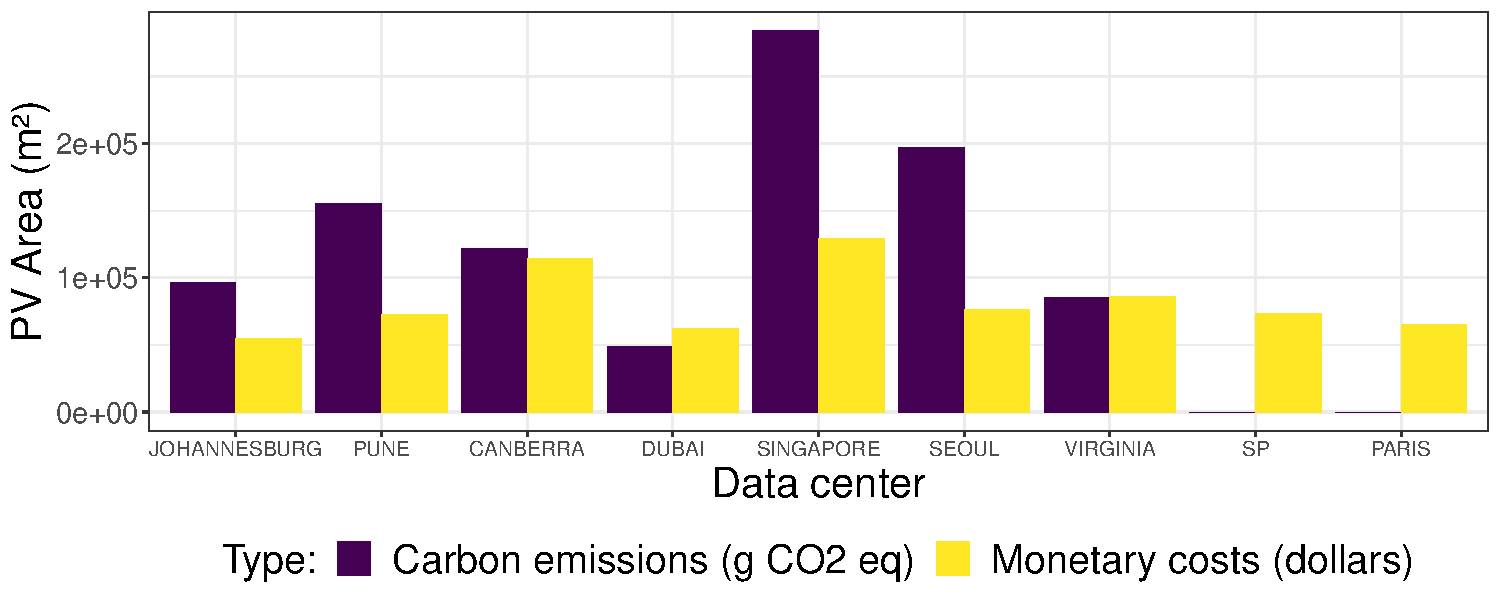
\epsfig{file = images/pv_sizing_co2_costs.pdf, width = .8\textwidth}}
  \caption{PV Area to minimize costs in comparison to minimizing carbon emissions. }
  \label{fig:pv_co2_costs}
\end{figure}


\begin{figure}[H]
  \centering
  {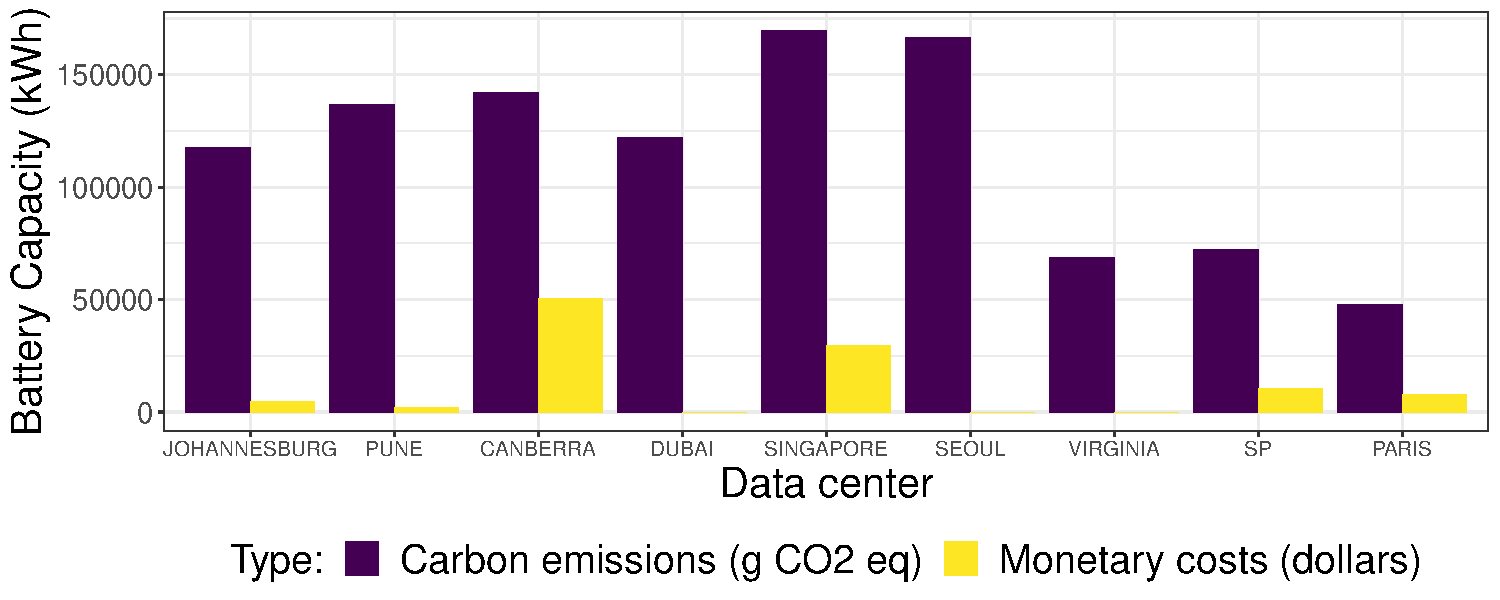
\epsfig{file = images/bat_sizing_co2_costs.pdf, width = .8\textwidth}}
  \caption{Battery capacity to minimize costs in comparison to minimizing carbon emissions.  }
  \label{fig:bat_co2_costs}
\end{figure}

\begin{figure}[H]
  \centering
  {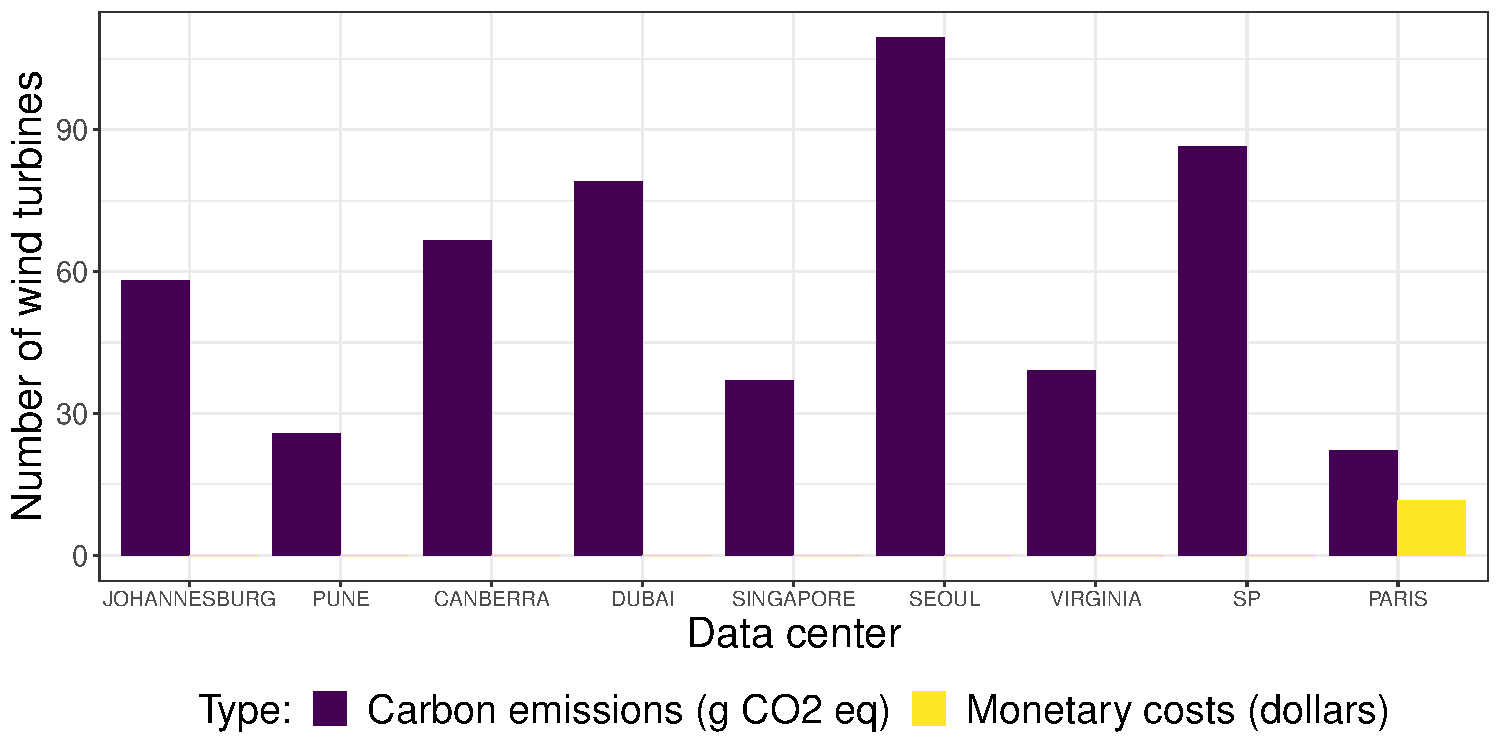
\epsfig{file = images/wt_sizing_co2_costs.pdf, width = .8\textwidth}}
  \caption{Number of wind turbines  to minimize costs in comparison to minimizing carbon emissions.}
  \label{fig:wt_co2_costs}
\end{figure}


\section{Adding or replacing servers considering new hardware and future workload }
\label{sec:new_servers}

In this section, we show the necessary modifications in our modeling to evaluate the decision to manufacture servers from new generations to match the cloud workload demand that increases year by year, considering that the servers also emit \ch{CO2} during their lifetime. It is assumed that the cloud federation will operate for the long term and that new servers will be launched during the lifetime of the cloud data centers. The decision-maker of the cloud federation will determine whether to add new servers to operate with the older ones from previous generations or to replace them, and can use forecasts of the cloud workload growth demand to guide the decision process.
\subsection{Updates in the model}

To model this approach, two new variables were created: $NS^d$, which represents the number of new servers to manufacture at the data center $d$; and $REP_{gen}^d$, the number of servers of the generation $gen$ to replace at the data center $d$. For replacing the servers from previous generations, it is considered that the data center computational capacity in the number of CPU cores cannot decrease, that is, the total number of CPU cores of the new servers needs to be greater or equal to the total number of CPU cores from the servers replaced. This constraint is modeled by Equation~\eqref{eq:dc_cpu_capacity}.

\begin{equation} \label{eq:dc_cpu_capacity}
 NS^d \times cpucores_{newgen} \geq \sum_{oldergen}  REP_{oldergen}^d \times cpucores_{oldergen}
\end{equation}

The number of servers replaced by a generation cannot be greater than the number of servers of this generation that exist in the DC ($ES_{gen}^d $). The value of  $ES_{gen}^d $ is extracted from the solution of the previous year. Equation~\eqref{eq:rep_only_existing_servers} models this constraint.

\begin{equation} \label{eq:rep_only_existing_servers}
 REP_{gen}^d \leq ES_{gen}^d 
\end{equation}


Given that a data center may have servers of different generations, it is also necessary to update the models regarding workload execution and power consumption. Now, we have a variable $w_{k,gen}^d$ that represents the workload that is executed on the servers of a generation $gen$ at the data center $d$ during a time slot $k$. We have two constraints for this variable: one for the servers that already exist in the DC, and another for the new servers that will be manufactured in the DC. Equation~\eqref{eq:workload_gen} models this constraint.


\begin{equation} \label{eq:workload_gen}
w_{k,gen}^d \leq   \left\{ 
  \begin{array}{ c l }
    (ES_{gen}^d - REP_{gen}^d) \times cpucores_{gen}  & \quad \textrm{if server from older generation  }     \\
     NS^d \times cpucores_{gen}   & \quad \textrm{if server from new generation  }      \\
    
  \end{array}
\right.
\end{equation}

Equation~\eqref{eq:wkgen} models the constraint that all the workload must be executed, and that it can be run on any generation of the servers.

\begin{equation} \label{eq:wkgen}
    w_k = \sum_{T_i|r_i\leq k\Delta t<r_i+p_i} c_i = \sum_d \sum_{gen} w_{k,gen}^d
\end{equation}

We also assume that the workload is classified into two categories: services that are mandatory tasks that execute in the DCs, and batch tasks that can execute in any of the DCs. This assumption represents the modern workload of cloud platforms and also avoids allocating all the workload to the DC with the lowest carbon-intensive grid and only adding and replacing servers on this DC. To model the classification of the workload into two categories, we need a new parameter $\gamma$ that represents the ratio of tasks that are of the service type (and 1 - $\gamma$ tasks are of the batch type) executed at each data center $d$. Equation~\eqref{eq:workload_category} models this restriction.

\begin{equation} \label{eq:workload_category}
 \sum_{gen}  w_{k,gen}^d \geq  w_k \times \gamma^d
\end{equation}


Equation~\eqref{eq:power_servers_gen} presents the new modeling of the power consumption for all the servers of different generations at a DC $d$, and Equation~\eqref{eq:power_cons_gen} models the power consumption of the DC (including the costs of the intra-network equipment and the cooling devices).


\begin{equation} \label{eq:power_servers_gen}
   PServers^d  =  \big(\sum_{gen} ES_{gen}^d \times  Pidle_{gen}^d + w^d_{k,gen}  \times  Pcore_{gen} \big)
\end{equation}


\begin{equation} \label{eq:power_cons_gen}
   P^d_k  = PUE^d \times \big(Pintranet^d + PServers^d\big)
\end{equation}

Regarding the carbon footprint of the servers, it is assumed that it is amortized over the server lifetime, and the LP considers the annual value. For example, if manufacturing a server emits 800 kg of \ch{CO2}-eq and its expected lifetime is 4 years, 25\% (200 kg of \ch{CO2}-eq) of its manufacturing emissions will be accounted for in the 1st year of operation, the other 25\% in the second year, and so on. After the fourth year, the server can still remain on the cloud platform, and its carbon emissions will come only from power consumption---all the carbon emissions from manufacturing have been amortized. On the other hand, if the server is replaced in the second year of operation, the remaining 75\%  of its emissions from manufacturing will also be taken into account. Equation~\eqref{eq:co2_new_servers} illustrates the footprint of building additional servers at a given data center $d$, where $serversCO2$ is an input with the total \ch{CO2} emitted from manufacturing the server (in $g\,\ch{CO2}\text{-}eq$), and $\epsilon$ the share of the emissions by year---$\epsilon$ is equal to 0.25 on the previous example.

\begin{equation} \label{eq:co2_new_servers}
FPns^d = NS^d \times (serversCO2 \times \epsilon)	
\end{equation}

Equation~\eqref{eq:co2_rep_servers} illustrates the footprint of replacing servers from previous generations at a given data center $d$, where $repCO2_{gen}$ is the emissions (in kg of \ch{CO2}-eq) from replacing the old servers that depend on the server age ($age_{gen}$) in years. The function that computes the value of  $repCO2_{gen}$  is defined in Equation~\eqref{eq:amortizedCO2}.

\begin{equation} \label{eq:co2_rep_servers}
FPrep^d = \sum_{gen} REP_{gen}^d  \times repCO2_{gen}
\end{equation}


\begin{equation} \label{eq:amortizedCO2}
repCO2_{gen} =  \left\{ 
  \begin{array}{ c l }
    (1 - (age_{gen} * \epsilon)) \times serverCO2   & \quad \textrm{if $age_{gen}$}  <  \textrm{expected lifetime}      \\
    0     & \quad  \textrm{otherwise}   \\
  \end{array}
\right.
\end{equation}


We also have the carbon footprint of the servers that were manufactured in previous years. Equation~\eqref{eq:co2_existing_servers} illustrates the emissions of the \textbf{e}xisting \textbf{s}ervers where $esCO2_{gen}$ represents the emissions of operating the server of the generation $gen$ during that year (in $g\,\ch{CO2}\text{-}eq$) and its value is computed by the function in Equation~\eqref{eq:serverCO2}.


\begin{equation} \label{eq:co2_existing_servers}
FPes^d = \sum_{gen} (ES_{gen}^d - REP_{gen}^d)  \times esCO2_{gen}
\end{equation}


\begin{equation} \label{eq:serverCO2}
esCO2_{gen} =  \left\{ 
  \begin{array}{ c l }
    \epsilon \times serverCO2   & \quad \textrm{if $age_{gen}$}    < \textrm{expected lifetime}   \\
    0     & \quad \textrm{otherwise  } \\
  \end{array}
\right.
\end{equation}

It is assumed that the renewable infrastructure stays the same from one year to another. Equations~\eqref{eq:low_bound_bat},  ~\eqref{eq:low_bound_pv} and ~\eqref{eq:low_bound_wt} model these constraints, where $lowboundbat^d$, $lowboundpv^d$ and $lowboundwt^d$ are the capacity of batteries, area of PVs and number of wind turbines, respectively, obtained from the sizing process.

\begin{equation} \label{eq:low_bound_bat}
Bat^d = lowboundbat^d
\end{equation}

\begin{equation} \label{eq:low_bound_pv}
A^d = lowboundpv^d
\end{equation}

\begin{equation} \label{eq:low_bound_wt}
WT^d = lowboundwt^d
\end{equation}


Finally, Equation~\eqref{eq:new_obj_co2_servers} presents the new objective function of operating the cloud platform, considering that new servers can be manufactured and servers from previous generations can be replaced.

\begin{equation} \label{eq:new_obj_co2_servers}
\text{minimize }\sum_{k=0}^{K-1} \sum_{d=1}^D (FPgrid^d_k +  FPpv^d_k + FPbat^d_k) + \sum_{d=1}^D   FPns^d + FPrep^d + FPes^d 
\end{equation}

\subsection{Experiments}


Two scenarios are considered in the experiments to assess the impact of the decision to manufacture new servers in terms of \ch{CO2} emissions. In the first scenario, the LP is solved only by having information on the current year's servers and the cloud workload growth forecast. This will generate a plan for the expected server lifetime---to consider all the carbon emissions from manufacturing. In other words, the LP is solved for four years -- starting from the year $x$---considering that it is only possible to manufacture the server of the current year that will be used together with the existing computational infrastructure or to replace older servers. 

Suppose a new, more computationally powerful and energy-efficient server is launched in the next year ($x+1$) or a new forecast for the workload growth for the following years is published. In that case, the initial plan of the previous year (year $x$) can be modified to consider information about the new server or a forecast of the workload growth. This will generate a new plan for the years $x+1$ to $x+5$. After the LP is solved for the year $x$, the results in terms of new servers manufactured and older ones replaced will be used as input to the year $x +1$. 

In the second scenario, the five years of operation are solved at once. Therefore, the LP has access to all the information about future workloads (the real growth), and server configurations. The first scenario represents an approach more realistic that has the potential to be taken by the decision maker, considering that it is hard to have accurate values for workload and server configurations in the long term, and the second scenario is only used as a baseline---it represents the optimal solution.

The two approaches----the greedy approach and the optimal---are compared using the metric total carbon emissions---originated from manufacturing the servers, the life cycle of the renewable infrastructure, and power consumed from the local grid.

\subsubsection{Settings}

We consider five years of operation and four generations of servers. For the workload growth, we assumed 22\% per year as reported by Cisco for the period 2017 to 2021~\cite{cisco_global_cloud_index_2018}---for each year, we use an input where the number of requested CPU cores per time slot to execute the workload is 22\% higher than the previous year. Regarding the server configuration, for each year from 2017 to 2021, we selected the server that had the highest score in the SPEC Power benchmark~\cite{spec_power}---a benchmark that assesses servers regarding both performance and energy---to represent the state-of-the-art. Table~\ref{tab:servers_specs} lists the differences in terms of hardware characteristics, power consumption, and the carbon footprint of manufacturing each server for the different generations. It is worth noting that in some cases, the same CPU was used in the servers that had the highest score for multiple years (such as the Intel Xeon Platinum 8180 and the AMD EPYC 7742). For the \ch{CO2} of manufacturing the servers, the methodology from the work of ~\citet{gupta2022_ACT} is used, which presents how to compute the carbon footprint of servers considering the integrated circuits of  RAM, storage (HD and SSDs) and CPU.

\begin{table}[h]
  \small
  \caption{Servers specifications for different generations. Values are inspired by results from the SpecPower benchmark \cite{spec_2014,spec_2017,spec_2016,spec_2019,spec_2021}.} \centering
  \label{tab:servers_specs} 
  \begin{tabular}{|l|r|r|r|r|r|}
  \hline    
  \textbf{Years} & \textbf{CPU} &   \textbf{Cores} & \textbf{Pidle}  & \textbf{Pcore}  & \textbf{$\mathbf{kg\,\ch{CO2}\text{-}eq}$}  \\
  \hline
  < 2016      & Intel Xeon E5-2660V2 & 20 & 52 & 7.5  & -   \\
  \hline
  2017, 2018  & Intel Xeon Platinum 8180 & 56 & 48.9 & 6.68  & 578.6   \\
  \hline
  2019, 2020   & AMD EPYC 7742  & 64 & 66.1 & 2.71  & 587.2 \\
  \hline
  2021        & AMD EPYC 7763 & 128 & 75.6 & 3     & 590.3 \\
  \hline
\end{tabular}  
\end{table}

All the servers are based on the Dell R740 for the HD and SSD values (HD with 3.84 TB and SSD with 400GB), with the same values for \ch{CO2} as in the work from ~\citet{gupta2022_ACT}, and they have 256 GB of RAM (16 modules of 16 GB DDR4 10 nm). For the CPU, the \ch{CO2} depends on the die area size, the processor size (in nanometers), and the number of chips in the server. Table~\ref{tab:cpu_specs} presents the specifications of the CPUs used to compute their carbon footprint, and it is assumed that each server has two chips. For the first generation (year 2013), it is considered that the servers have been used more than their expected lifetime, and all their \ch{CO2} footprint has been paid. Finally, according to ~\citet{datacenter_as_computer}, the typical lifespan of servers is three to four years. Therefore, we consider the server's expected lifetime to be four years.


\begin{table}[h]
  \small
  \caption{CPU specifications in terms of die area and processor size. Values retrieved from x86guide.net \cite{ref_amd_epyc_7742,ref_amd_epyc_7763,ref_xeon_platinum_8180}.} \centering
  \label{tab:cpu_specs} 
  \begin{tabular}{|l|r|r|}
   \hline

  \textbf{Model}  & \textbf{CPU die area (cm²)} & \textbf{Processor size (nm) } \\
  %  \hline
   % Intel Xeon E5-2660V2 & 3.41  & 20  \\
   % \hline
   %Intel Xeon E5-2699 v3& 6.62  & 20  \\
   % \hline
   % Intel Xeon E5-2698 V4 & 4.56 & 14\\
    \hline
    Intel Xeon Platinum 8180 & 6.94 & 14\\
    \hline
    AMD EPYC 7742  & 5.92 & 7 \\
   \hline
    AMD EPYC 7763 & 6.45   & 7 \\
%    \hline
  %  AMD EPYC 9654 & 8.66 & 5 \\
  \hline
\end{tabular}  
\end{table}

To obtain the area of solar panels, the capacity of batteries, and the number of wind turbines, the sizing process was realized using the average irradiation and wind speed from 1980 to 2019, as in Section~\ref{sec:settings_wt}, and the server configurations of the year 1. For the remaining five years of operation, the wind speed data and solar irradiation used are from 2013 to 2017.
\subsubsection{Results}

Figure \ref{fig:dc_evolution_comparison} provides a comparison of both approaches---greedy and optimal methods---to deciding to manufacture new servers.   This comparison assesses the evolution of the cloud federation infrastructure in terms of computational power and which server generations are being used. The year 2016 represents the initial state of the cloud federation, which exclusively contains servers from the first generation. These servers had been in operation for a duration sufficient to offset all the carbon emissions associated with their manufacturing. The years 2017 to 2021 represent the five years of operation during which the two approaches for deciding whether to manufacture new servers are applied. 

Each bar in the figure represents the computational capacity of the cloud federation---quantified by the total number of CPU cores across all data centers. The colors denote the server generation of the CPU cores  (more recent generations have darker colors). One can also observe when new servers are added---the bar's height of the corresponding generation increases---and when servers from older generations are replaced with newer ones---the bar's height of the corresponding generation decreases. We also present the results of the decision to manufacture new servers for each DC in Figure \ref{fig:dc_evolution_year_by_year}---for the greedy approach---and Figure \ref{fig:dc_evolution_optimal}---the optimal solution.

We observe that the optimal solution makes very few changes to the servers, because it knows in advance when the right moment is to add or replace them and how . However, in real life, the first approach, where the decision is made year by year, is closer to what the cloud-federation operator would do. Finally, in terms of total \ch{CO2} emissions, the optimal solution is 13.4\% better than the solution that only has information about the current year, as can be seen in Table~\ref{tab:emissions_sizing}.

\begin{figure}[ht]
\centering 
  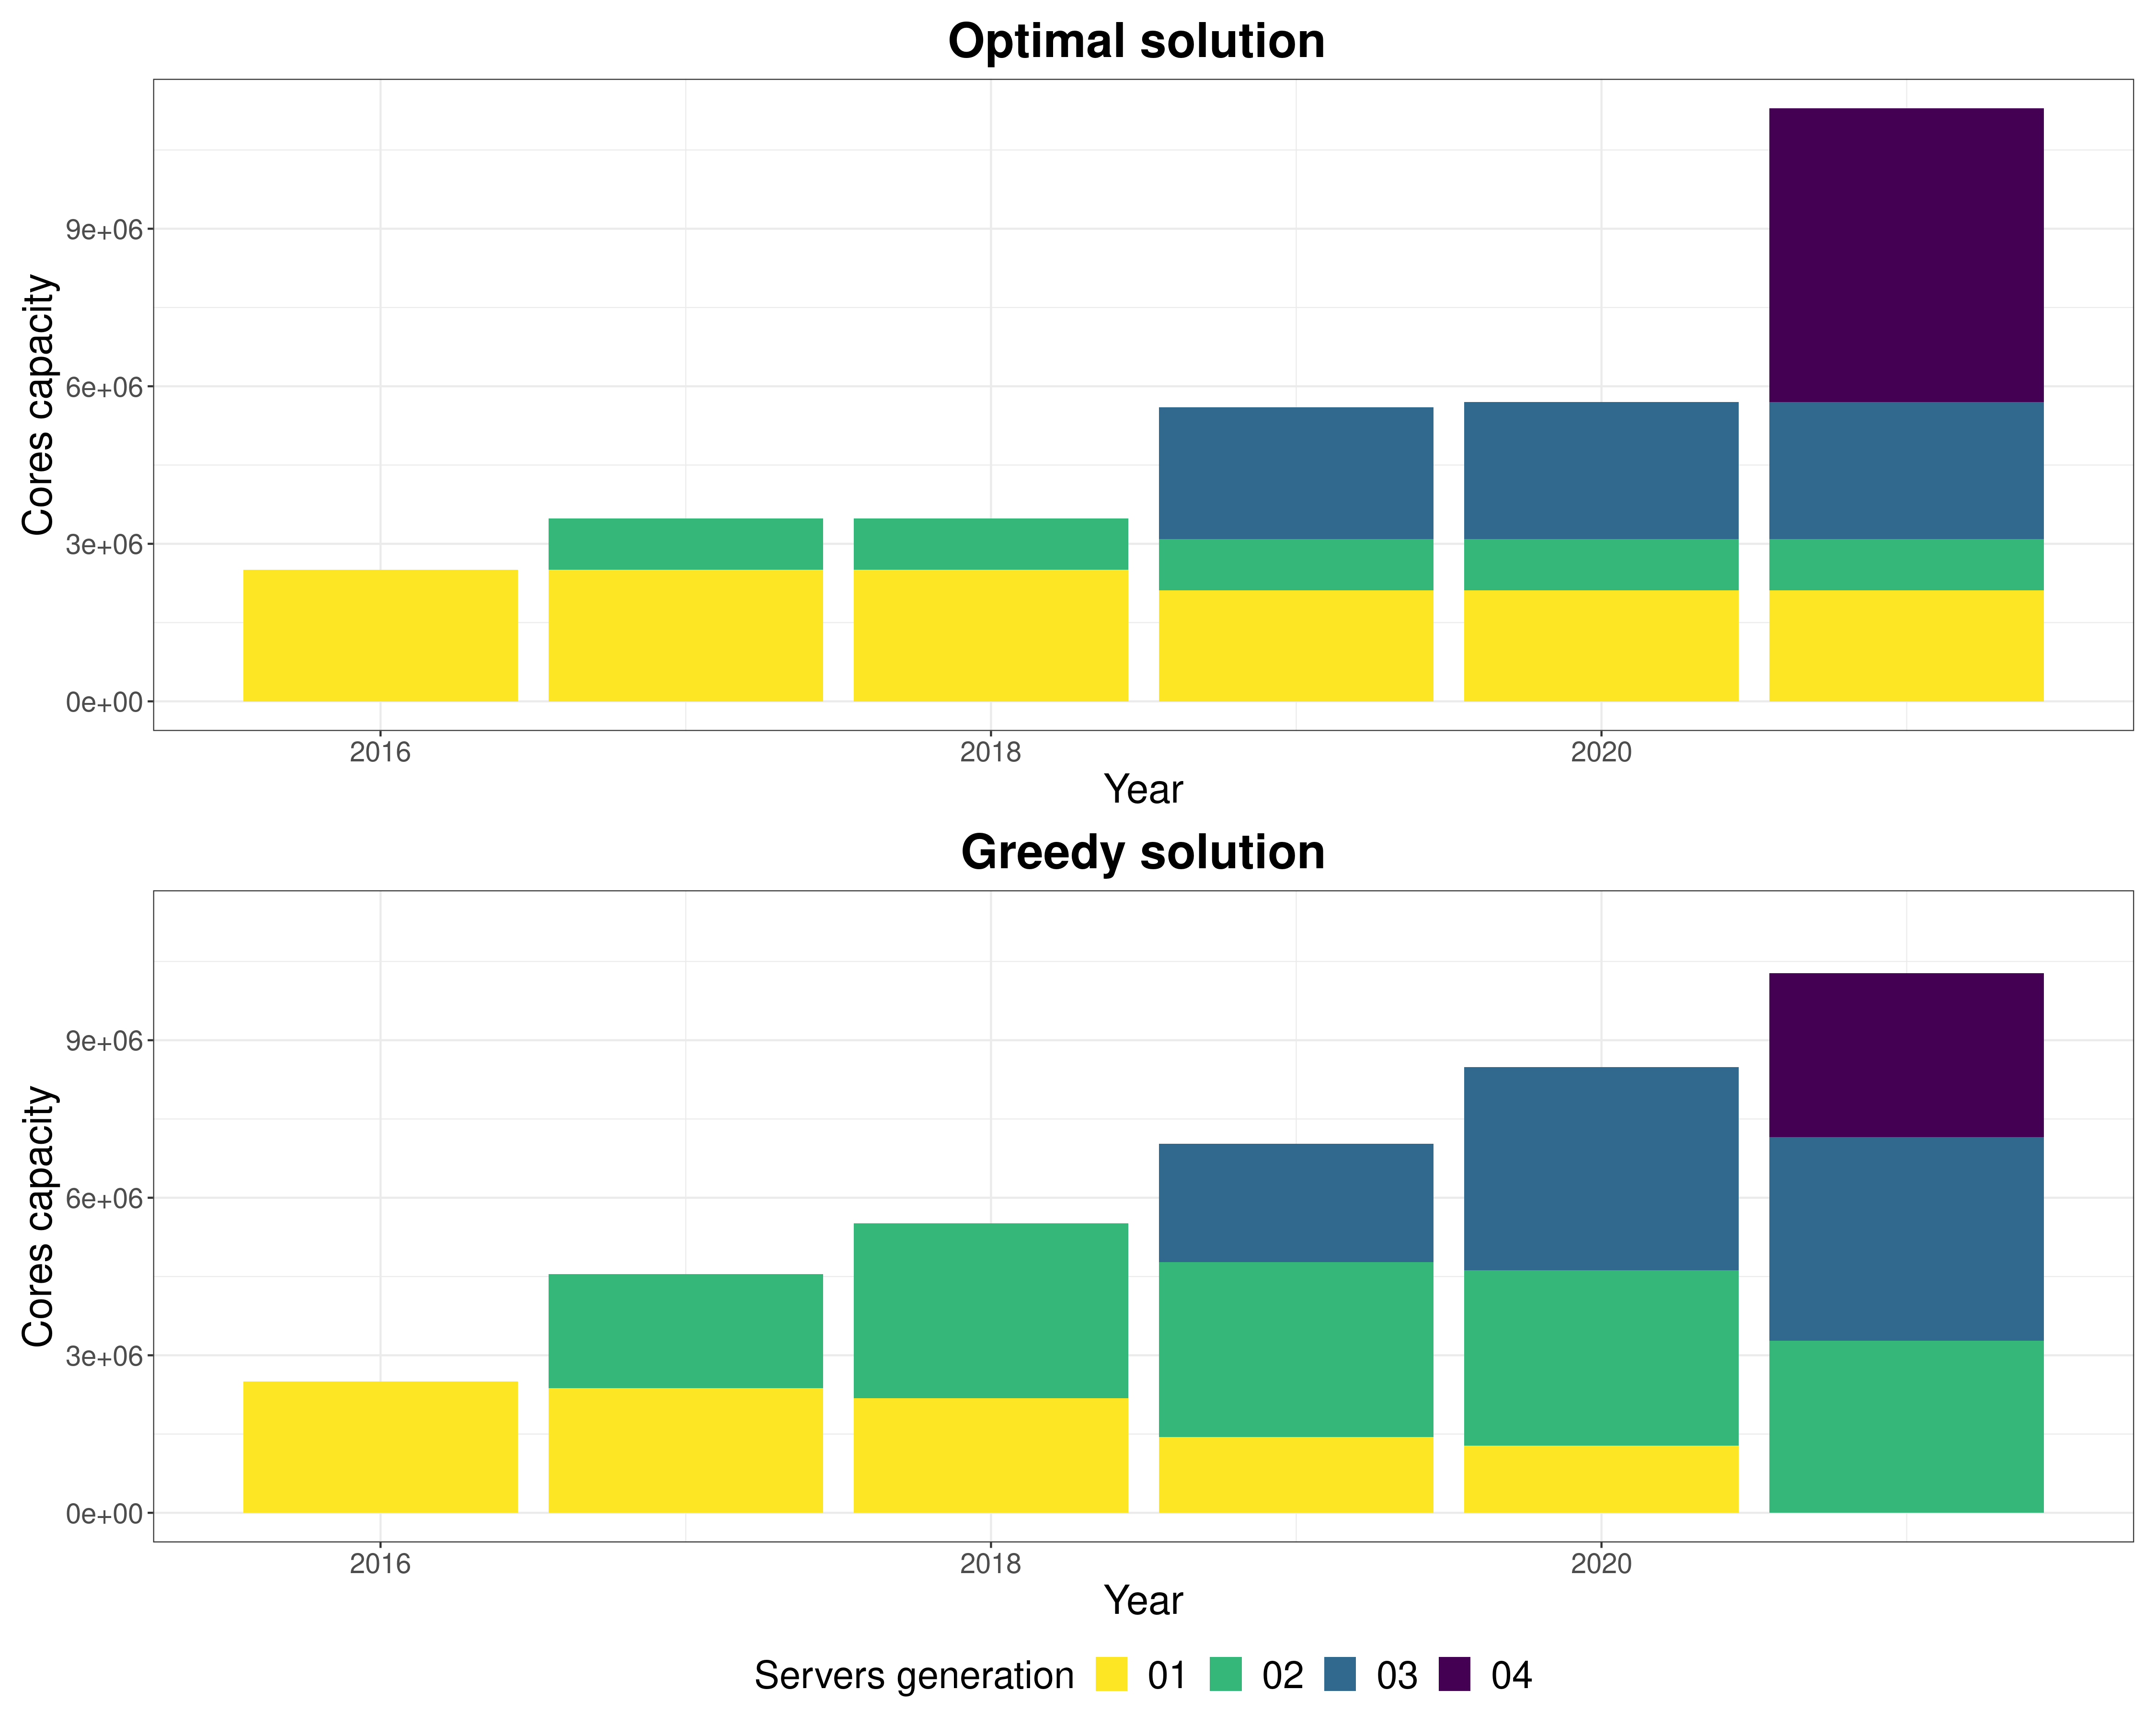
\includegraphics[width=\linewidth]{images/cloud_federation_evolution_lifetime.png}
  \caption{Comparison between the optimal and greedy approaches to decide manufacturing new servers in terms of total CPU cores of the cloud federation and the generation of servers.}
  \label{fig:dc_evolution_comparison}
\end{figure}


\begin{figure}[ht]
\centering  
  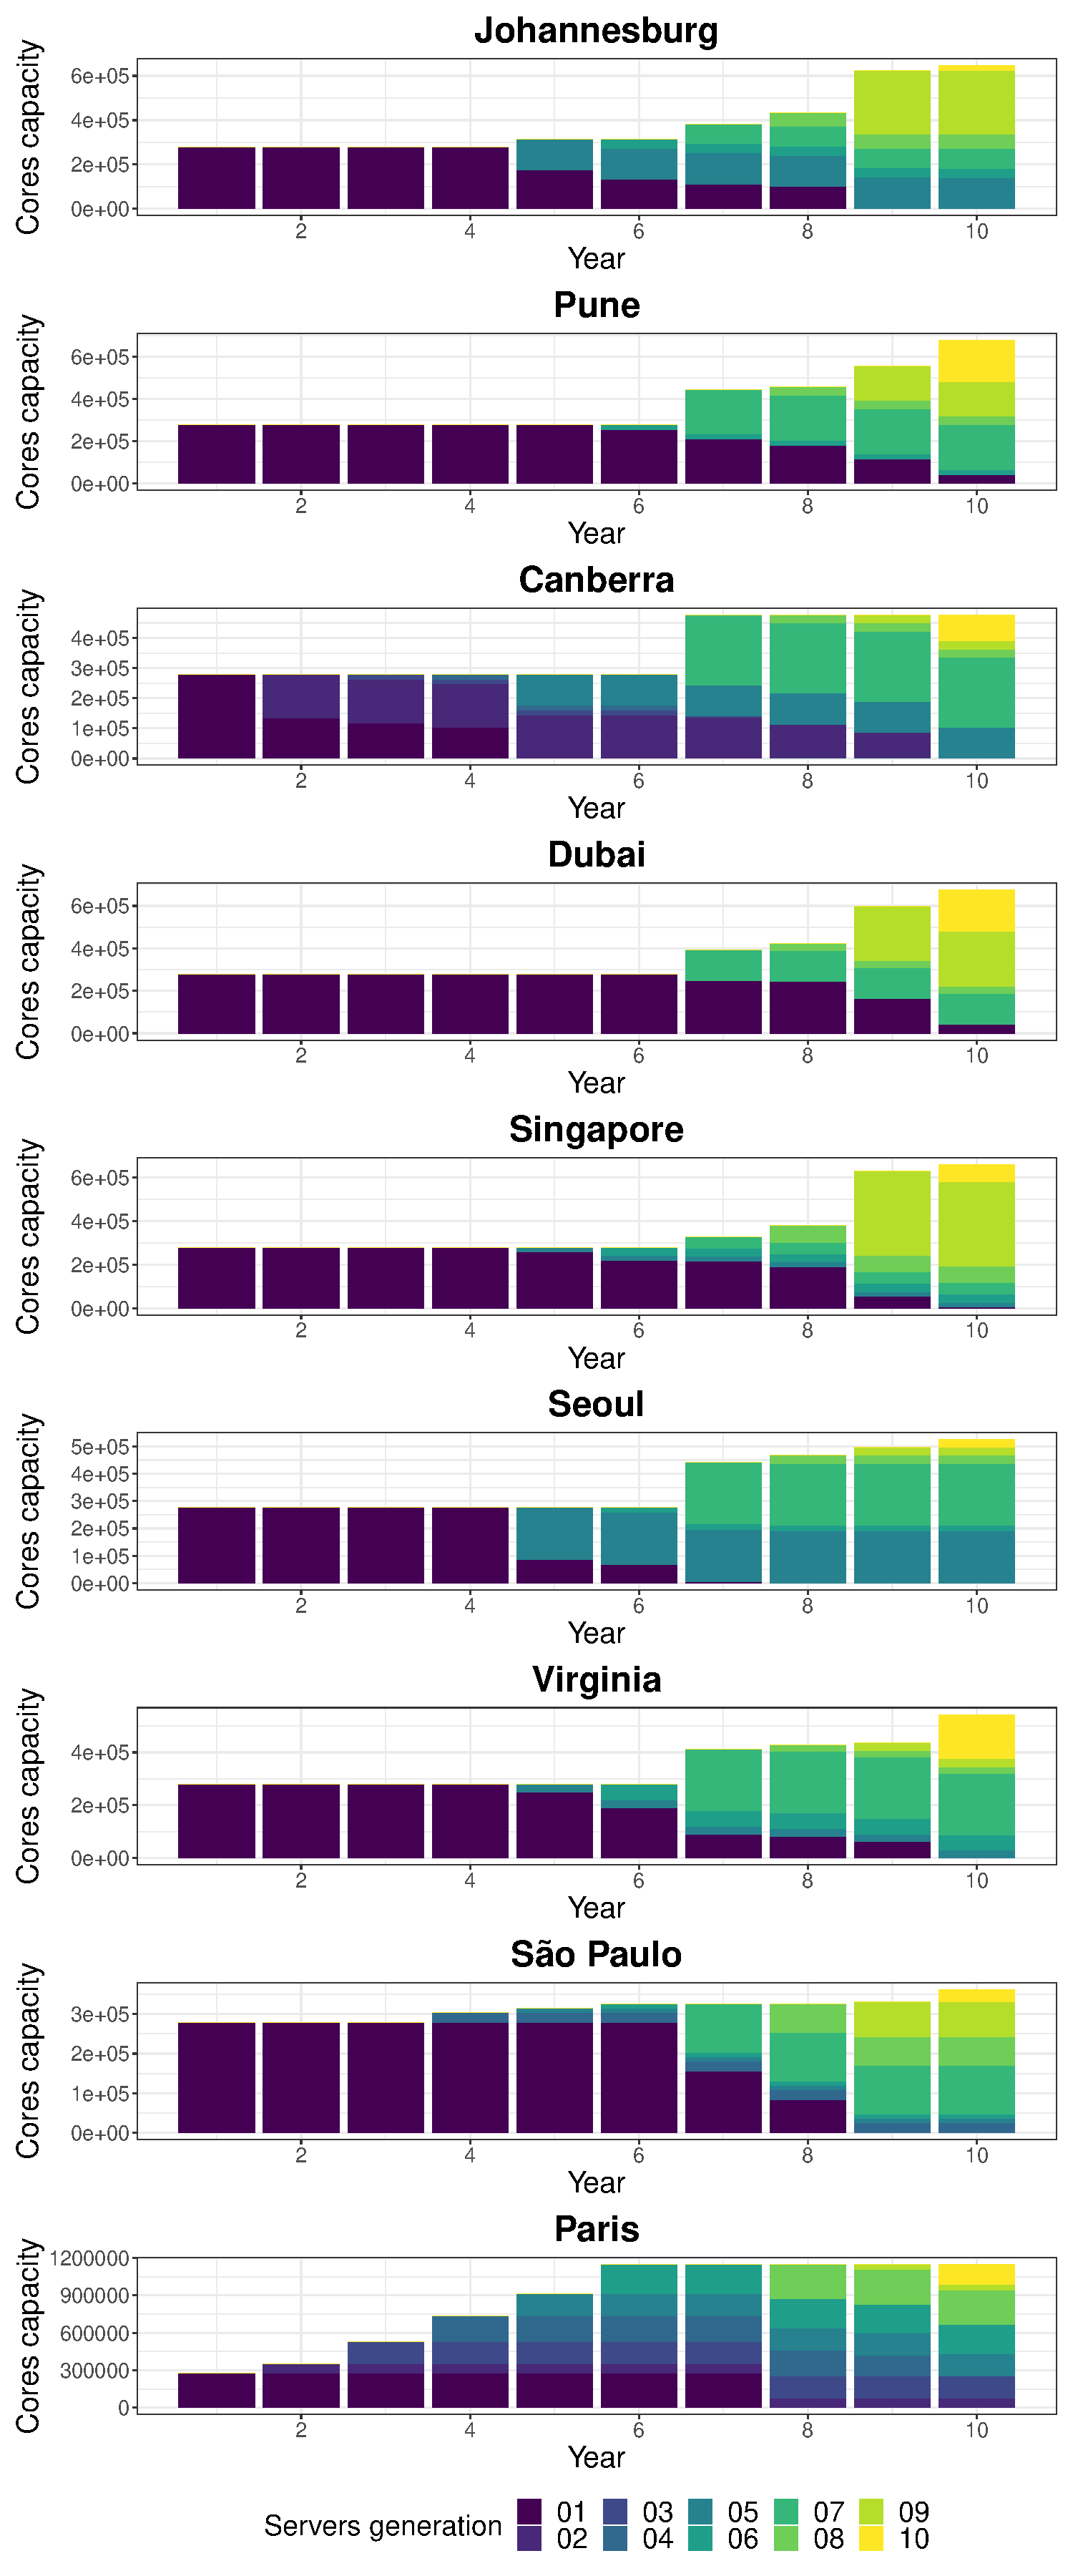
\includegraphics[width=\linewidth]{images/dc_evolution_year_by_year.pdf}
  \caption{Solution for the greedy approach to decide manufacture servers---when there is only access to information of the current year's server.}
  \label{fig:dc_evolution_year_by_year}
\end{figure}

\begin{figure}[ht]
\centering
  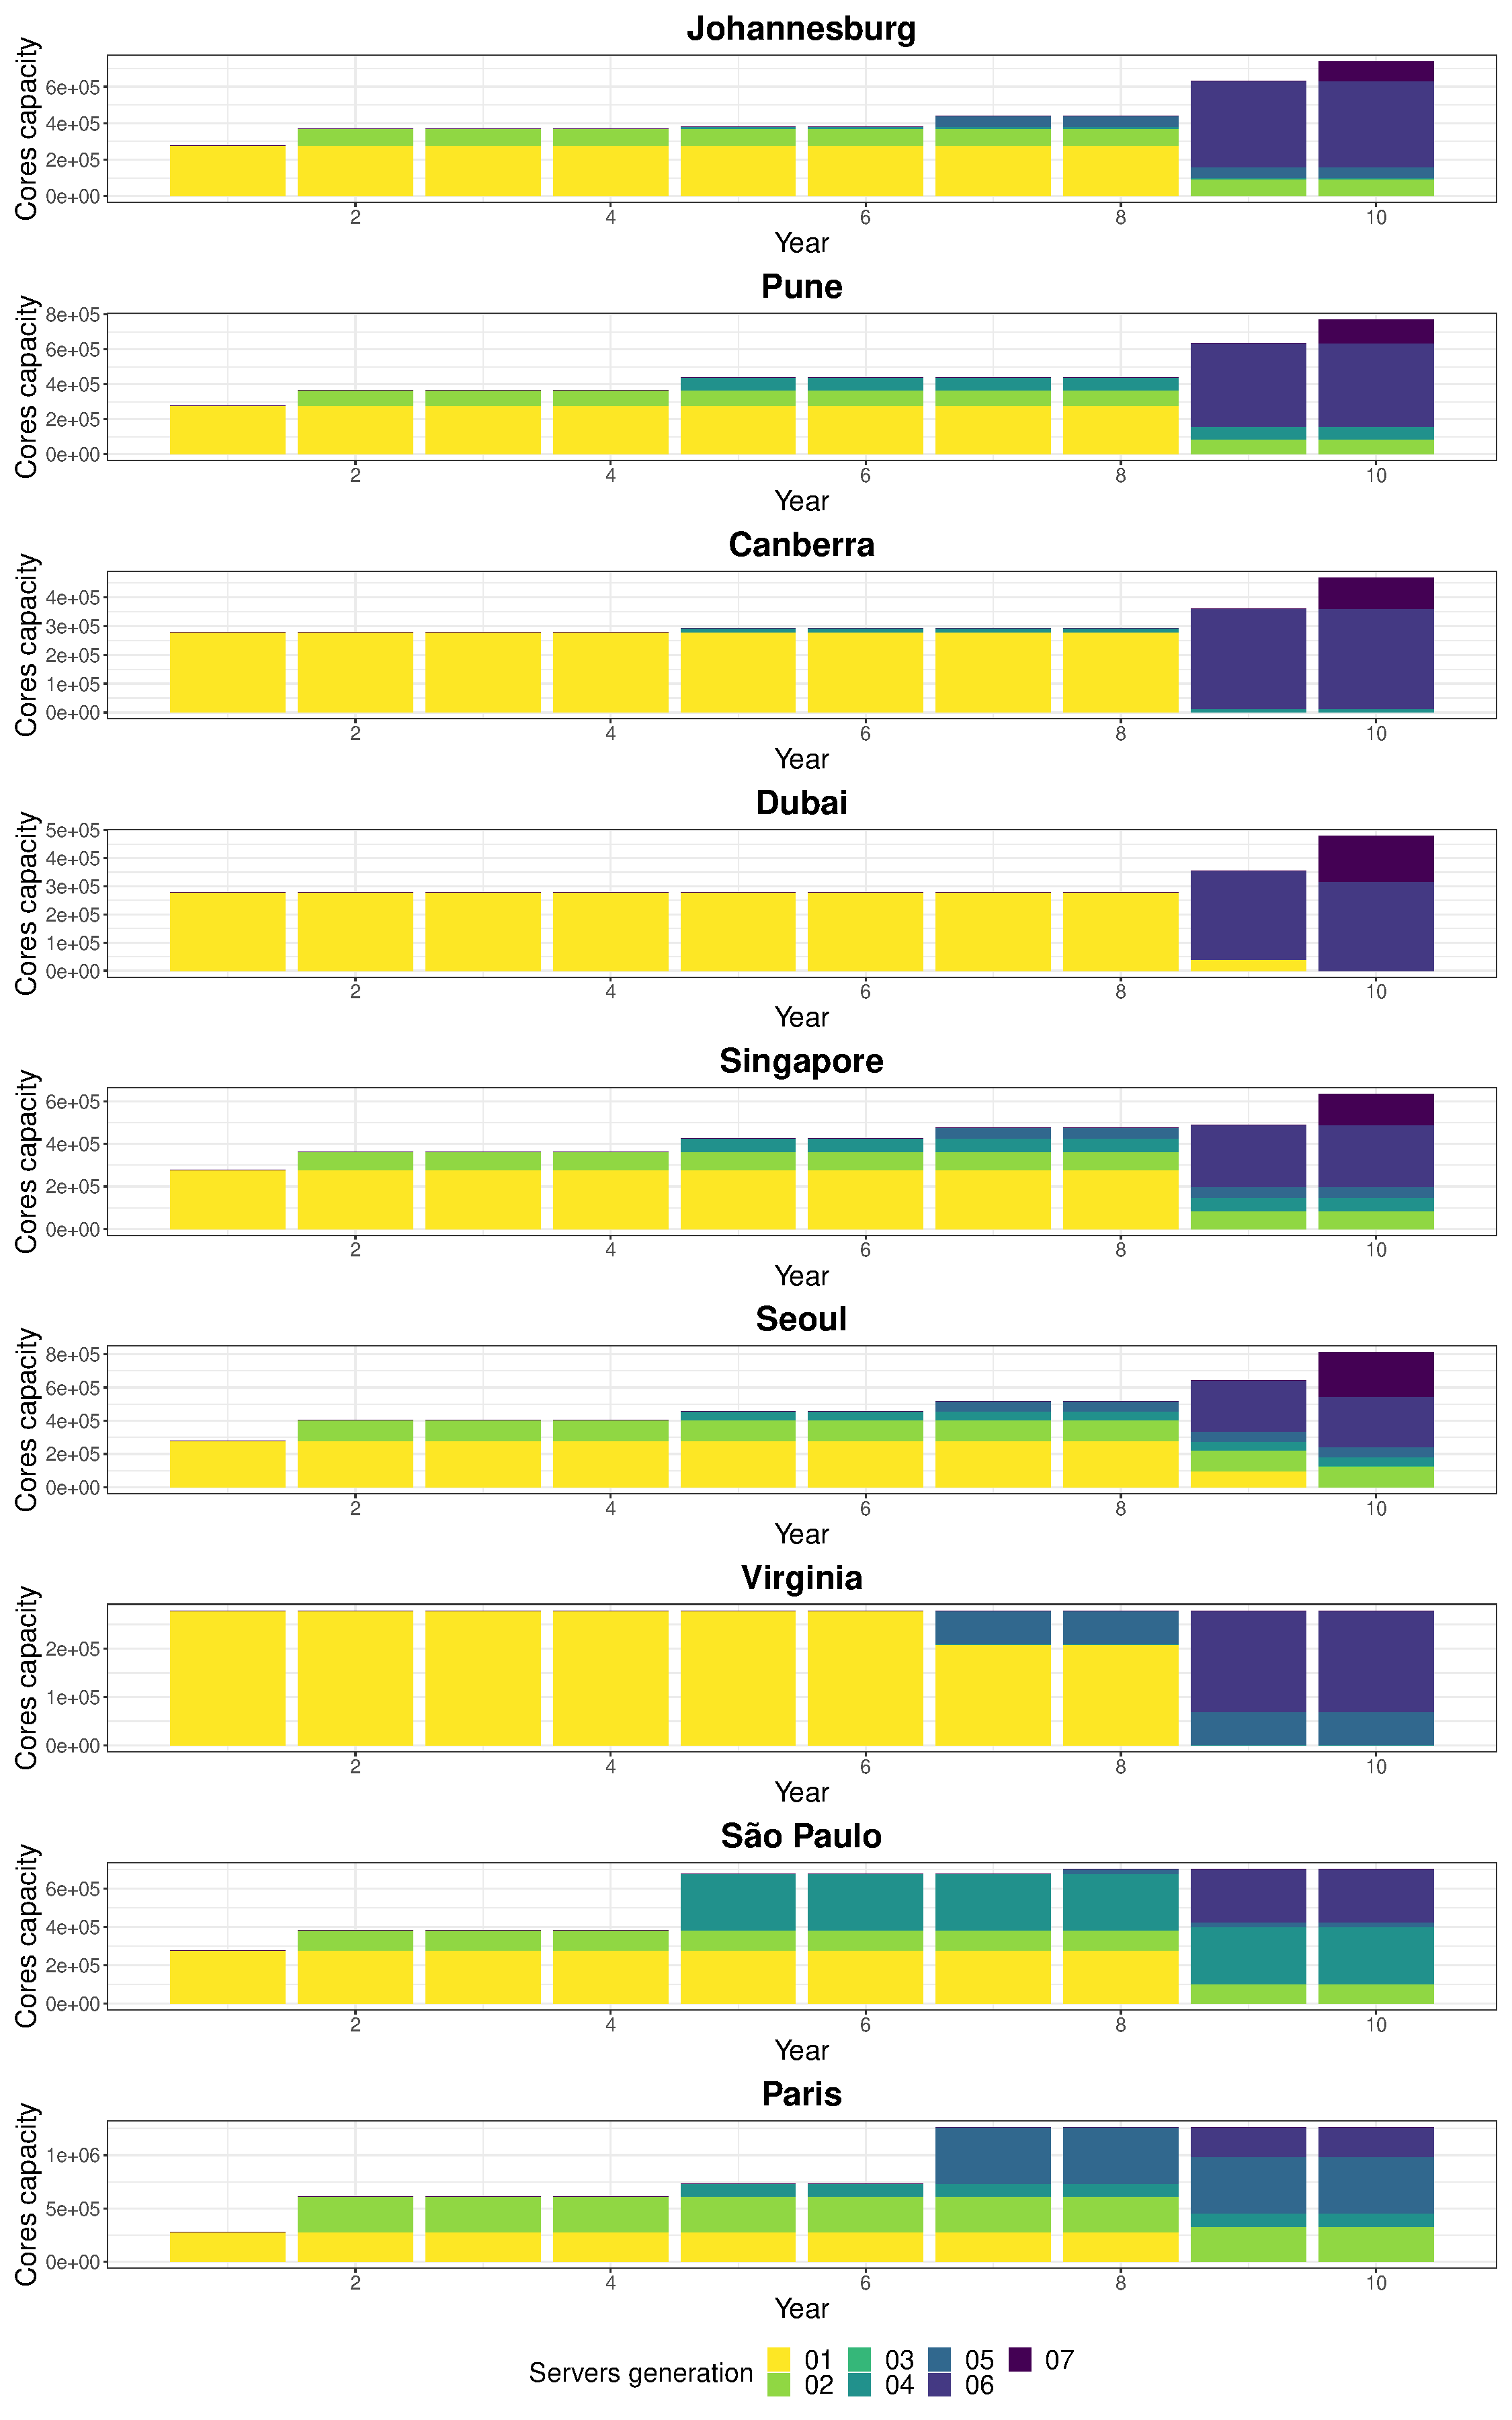
\includegraphics[width=\linewidth]{images/dc_evolution_optimal.pdf}
  \caption{Solution for the optimal approach to decide manufacture servers---when there is only access to information of the servers off all the years in advance.}
  \label{fig:dc_evolution_optimal}
\end{figure}


\begin{table}[!ht]
  
\caption{Total emissions for the different approaches to manufacture new servers.}\label{tab:emissions_sizing} \centering
\begin{tabular}{|l|r|}
  \hline
  \textbf{Scenarios} & \textbf{Emissions ($\mathbf{t\,\ch{CO2}\text{-}eq}$)}   \\
  \hline  
   Optimal solution  &   246 867.03 \\  
  \hline
   Greedy approach                   &   213 730.59  \\
  \hline

\end{tabular}
\end{table}


% To better understand how the data centers are being used over time, we present in Figures~\ref{fig:dcu_evolution} the average data center usage over the years, and the average ratio of the workload each data center received throguh the years ~\ref{fig:w_ratio_evolution} .


% \begin{figure}
%\centering
 % 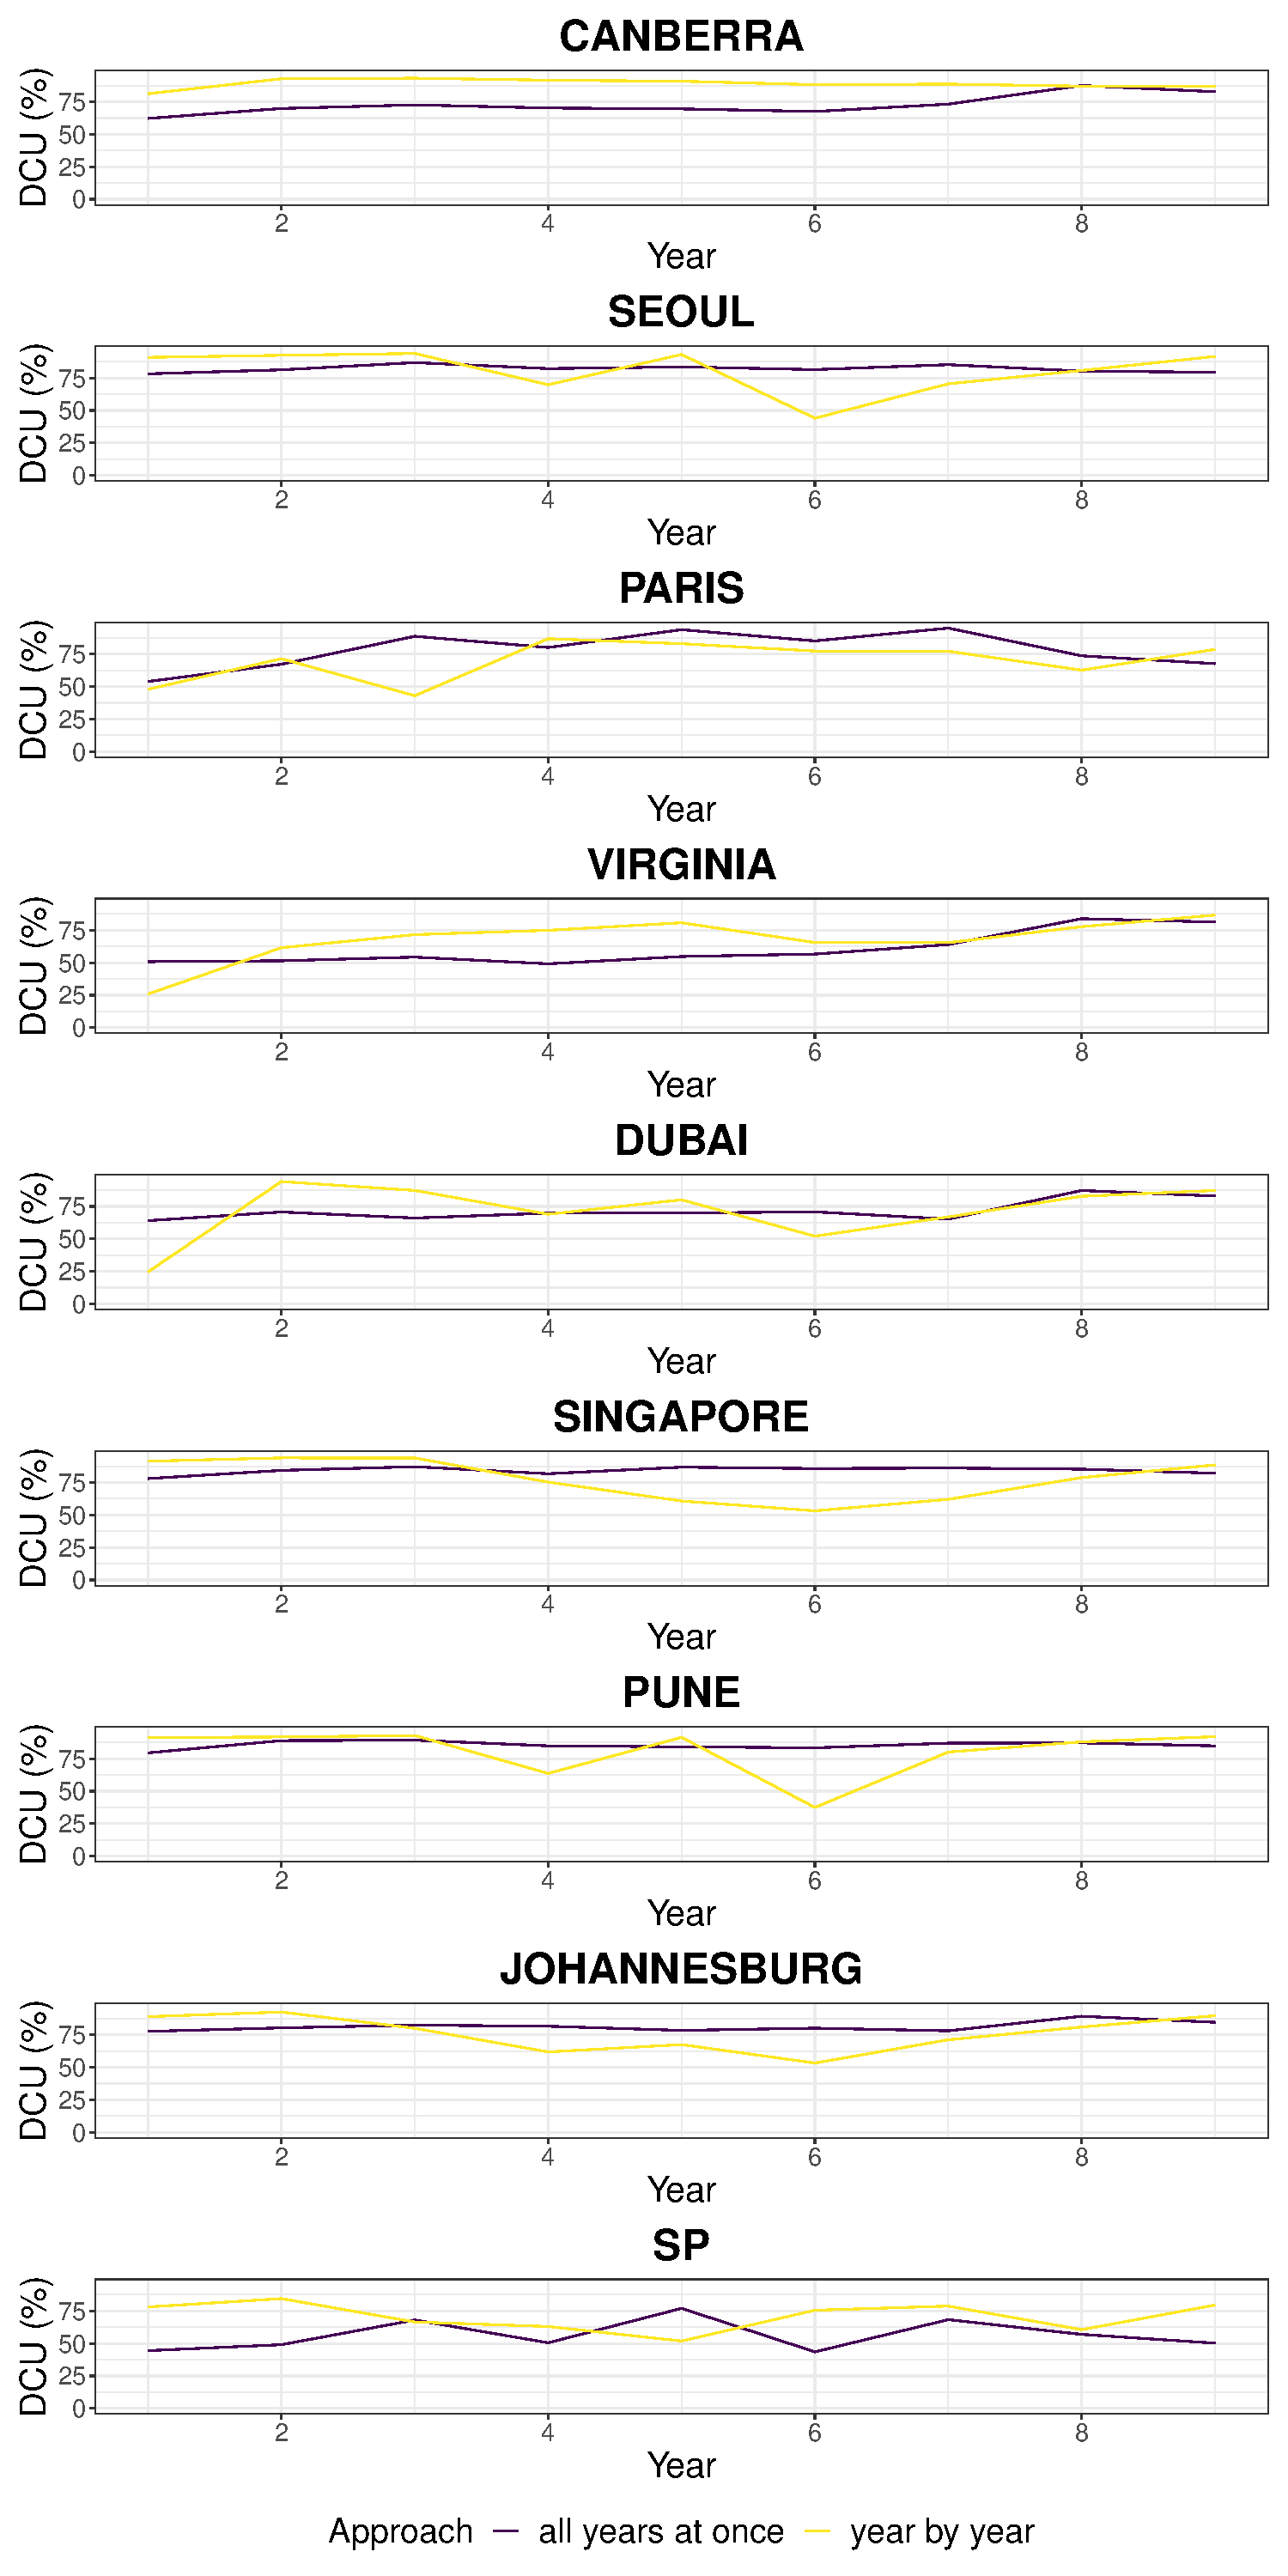
\includegraphics[width=.8\linewidth]{images/dcu.pdf}
  %\caption{Data Center Utilization  (DCU) comparison for the scenario where the decision to add new servers is made knowing all the information of the 10 years in advance and year by year.}
 % \label{fig:dcu_evolution}
%\end{figure}

%\begin{figure}
%\centering
 % 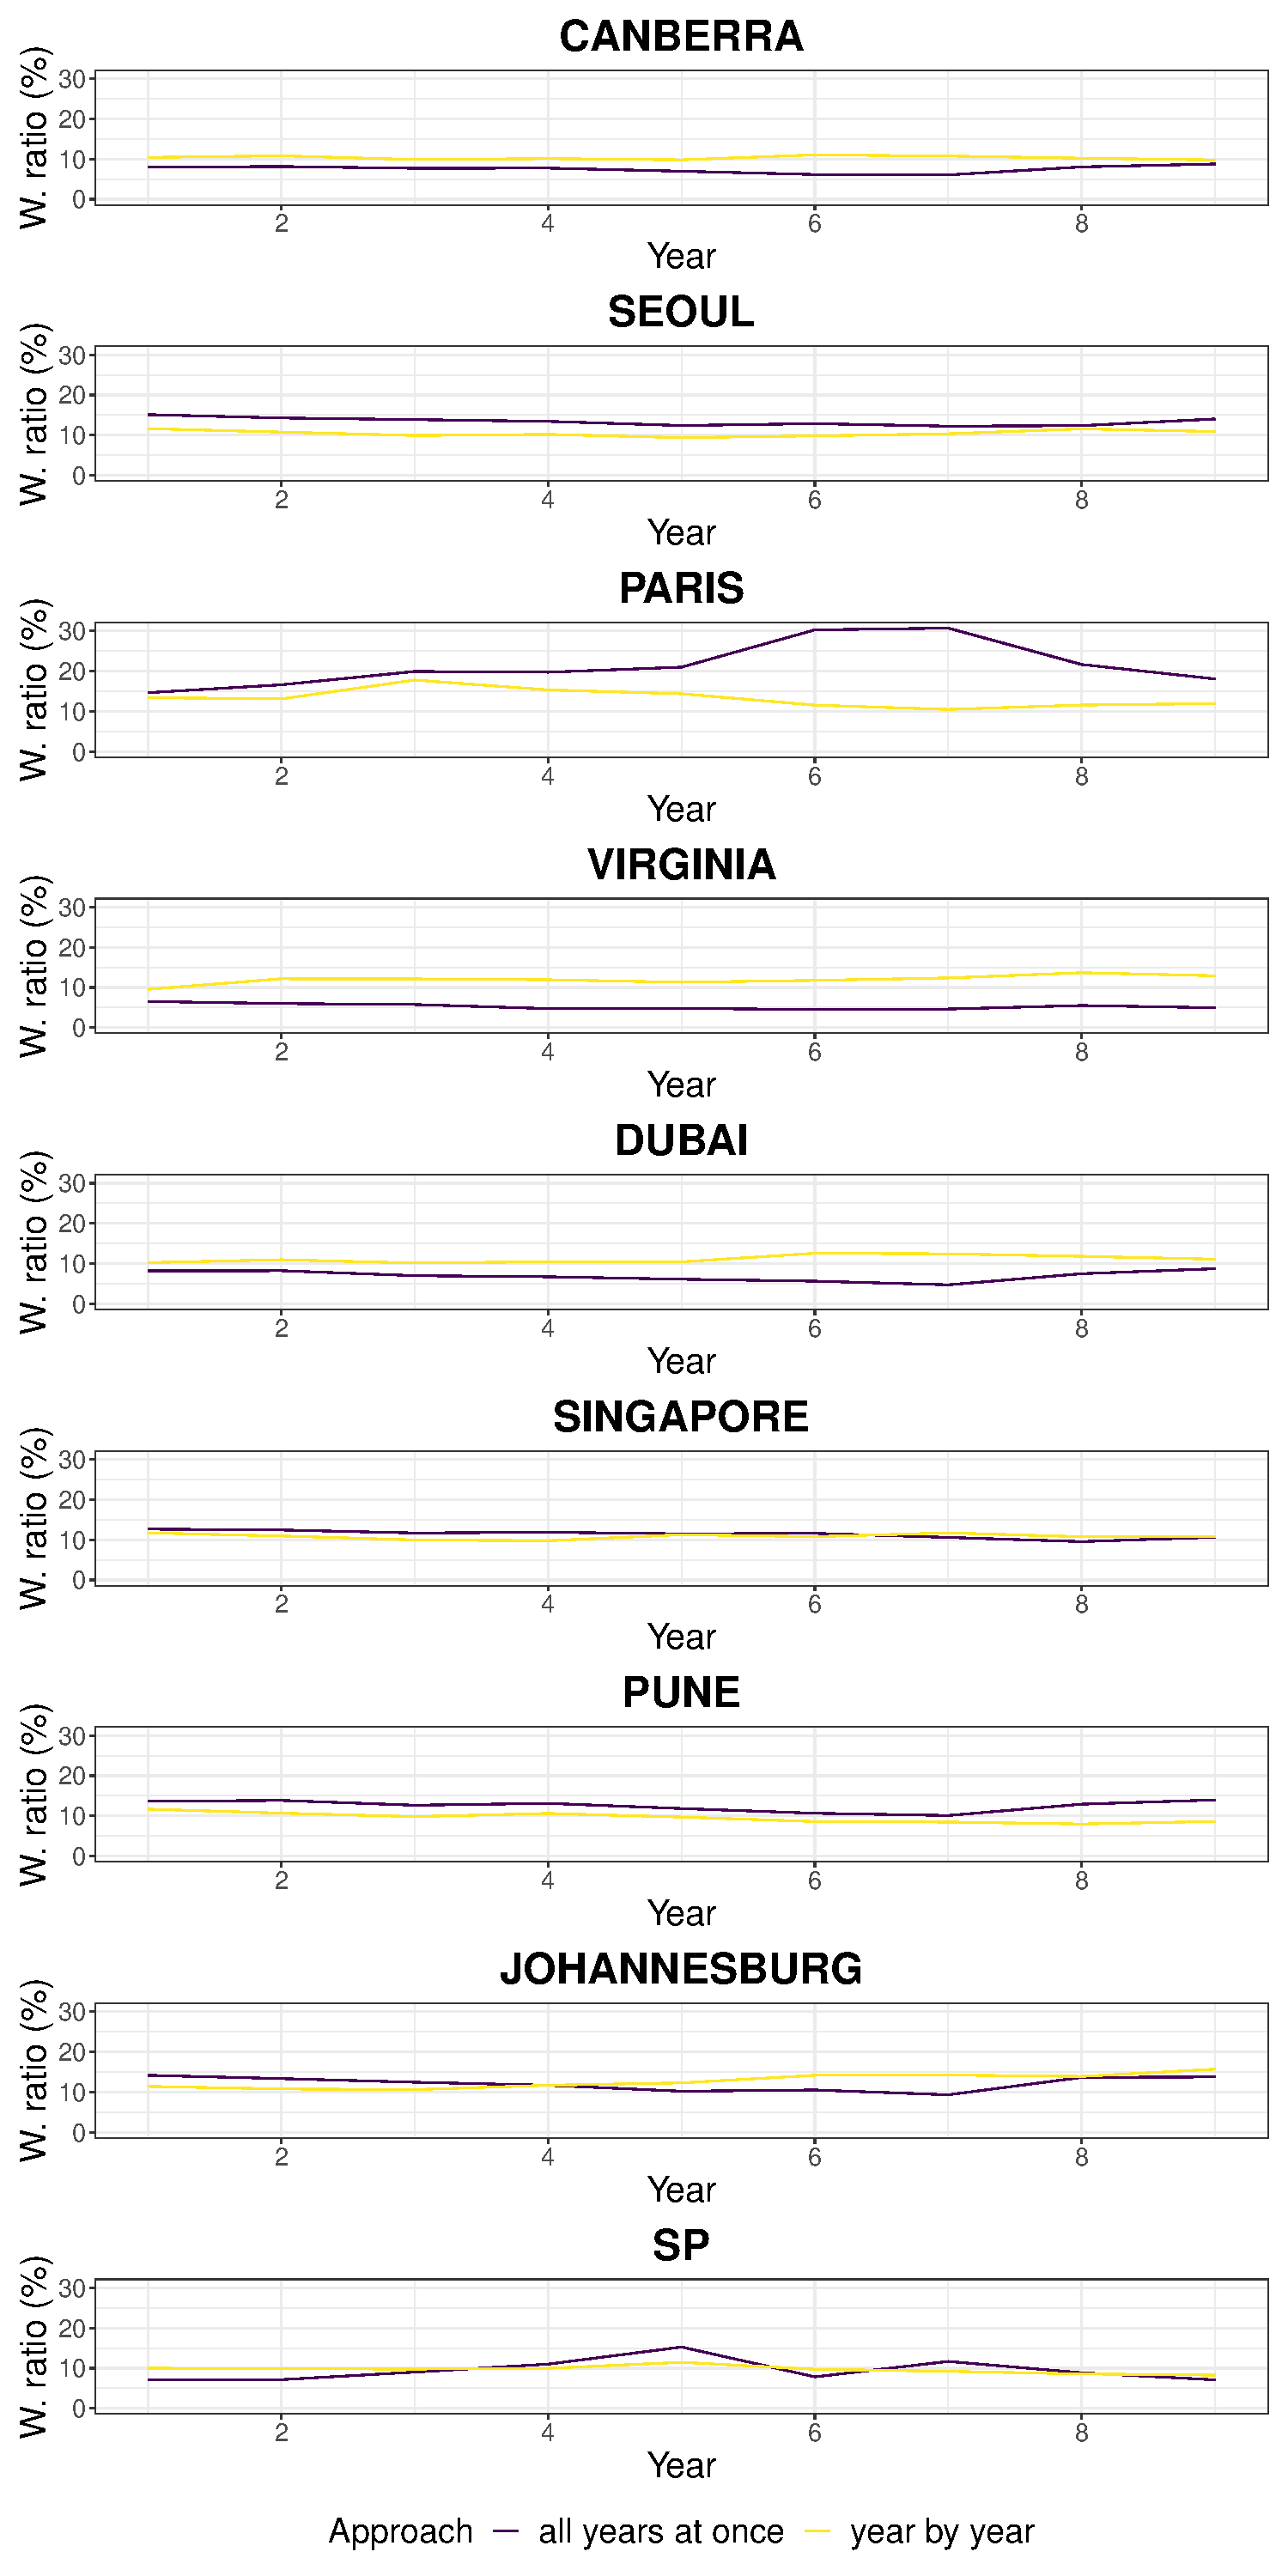
\includegraphics[width=.8\linewidth]{images/w_ratio.pdf}
  %\caption{Data Center Utilization  (DCU) comparison for the scenario where the decision to add new servers is made knowing all the information of the 10 years in advance and year by year.}
 % \label{fig:w_ratio_evolution}
%\end{figure}


%%% Add dcu, workload ratio e outras paradas ...


%%% co2 de servidores por ano                ...


%% Add figura de q o otimo considerando varios anos aleatorios n muda as emissoes ....


\section{Discussion}
\label{sec:long_term_discussion}

This section presents the reader with an analysis of the experiments and their results. The scope of the study is how to reduce the environmental impact that comes from the long-term operation of a cloud federation---in terms of \ch{CO2} emissions---by adding locally installed renewable infrastructure: solar panels, wind turbines, and batteries (to deal with intermittency). One must pay attention to the fact that renewable infrastructure also emits carbon throughout its lifetime. 

We made the modifications in our modeling---that initially only considered emissions from manufacturing---and, as expected, there was an increase in the total emissions---around 8\%. It is also possible to observe that the area of PVs was reduced in most of the locations---Figure ~\ref{fig:pv_lca}, except for Johannesburg. This could be explained by the fact that Johannesburg is the location that receives the most solar irradiation throughout the year, so it could compensate for the decrease in PV area in the other locations. Regarding the batteries, the reduction in Pune, Seoul, and Singapore could be justified by the smaller PV area, as there will be less energy to store.

On the other hand, we see an increase in battery capacity at the other locations. This could be justified by having a smaller PV area so the renewable energy cannot be wasted. Finally, including the life cycle aspect makes our modeling more realistic, and the emissions are still better than the scenario where only power from the local electricity grid is used in terms of carbon footprint---81\% in the scenario with PV and batteries.  


% Talk about adding wind turbines
Regarding the wind turbines, we saw that including them in the renewable infrastructure has a significant positive impact on the carbon footprint of operating the cloud federation: a 34\% reduction in \ch{CO2} emissions in comparison to only using solar panels and batteries. This reduction could be justified by the fact that renewable power is produced even when the sun is not shining and throughout the whole year, which results in a reduction in the required PV area and battery capacity that can be observed in Figures~\ref{fig:wind_pv} and ~\ref{fig:wind_bat}---in the previous chapter, we saw the dimensions of PV and batteries needed to deal with the low solar irradiation during winter.

Nevertheless, the number of necessary wind turbines to manufacture is quite high, and this is a problem considering the land area requirements of wind turbines. One study from NREL that evaluated the land area requirements in the United States reports that the average capacity density (relation between wind power production and required land area) is 3.0 ± 1.7 MW/km² \cite{wtlanduse_2009}. Taking into account that in our experiments, we considered wind turbines with a rated power of 1.5MW, this implies that for each square kilometer, it is possible to install from one to three wind turbines. This would not be possible for data centers located in urban centers that are highly populated. For example, in the case of Paris---the one with the lowest number of wind turbines---we would need from 7 to 23 km², and in the case of Seoul---the one with the highest number of wind turbines---it would require 36 to 110 km². 

In comparison to solar panels, we observe that for all the evaluated locations---except Paris---the wind turbines have a lower potential for power generation---as seen in the Capacity Factor values of Table~\ref{tab:capacity_factor}. Taking into account these points, it may be more interesting for the cloud federation operator to buy power from wind farms located near its data centers than to install wind turbines on them.

% talk about sizing sensitivity

As said in Section~\ref{sec:add_wt}, solar irradiation has a lower variance than wind speed, impacting the sizing process's quality. We saw that in the comparison of the optimal scenario for the renewable infrastructure that only considered PV panels and batteries, the sizing process that used simple estimation techniques (average and median values) had precise results, being up to 3\% worse than the optimal scenario (Table ~\ref{tab:co2_10y_pv_only}). On the other hand, the scenario that only considers wind turbines and batteries as the green power infrastructure (Table ~\ref{tab:co2_10y_wt_only}) was significantly worse when compared with the optimal solution---around 11\%---and presented more than two times the carbon emissions of only using solar panels---which can be justified by the lower potential to generate wind power on the selected locations as seen in Table~\ref{tab:capacity_factor}. 

For the scenario with a hybrid configuration of solar panels and batteries, it is possible to observe in Table ~\ref{tab:co2_10y_pv_only}) that it became less precise---up to 12\% worse than the optimal---as it is affected by the uncertainties of solar irradiation and wind speed. Nevertheless, even in the worst case, the reduction in total \ch{CO2} emissions by using the hybrid configuration with PVs and WTs is significant: the worst scenario for PV + WT + Bat has a 17\% lower carbon footprint than the scenario with PV + Bat.

% Granularity of emissions

In what concerns the sensitivity of the model to the grid emissions input, we saw that the initial modeling that uses the average value of the year is robust: using the hourly value reduces the total \ch{CO2} emissions by less than 1\%---as seen on Table~\ref{tab:co2_grid_granularities_years}. This result presents a positive outcome, considering that not every location provides a fine-grain value of the carbon intensity of its electricity grid.

% Talk about flexibility in the scheduling
On the topic of exploring the flexibility in the scheduling of the workload to reduce carbon emissions, it is possible to extract the following information from the results. The first is that the reduction of the carbon footprint seems to have a limit (around 4\%). This can be justified by the fact that there is little difference in the climate conditions during the interval of one week, or that the DC, which would reduce carbon emissions, is already at peak capacity and cannot receive more workload. 

The second interesting observation is that by delaying a small portion of the workload (for example, 10\% to 20\%)  the reduction is already really close to the maximum possible reduction value. Finally, this approach can be used to reduce the impact of renewable sources' intermittency in the sizing process---as we saw differences from 1\% to 12\% in comparison to the optimal scenario on Section~\ref{sec:sensitivity}---and in the context of cloud federations that emit from tens to hundreds of kilotons of \ch{CO2}-eq, a reduction of 4\% is not negligible.

% Talk about costs
Concerning the costs of reducing the environmental impact of the cloud operation---one of the most important variables for the decision-makers---we see in Table~\ref {tab:total_price_and_co2_grid_timeseries} that the hybrid configuration that uses solar panels and wind turbines is the cheapest---around 35\% cheaper and emits 37\% less \ch{CO2} in comparison with using only the grid. On the other hand, the solution that results in the lowest environmental impact (\textit{Minimum \ch{CO2} PV + WT + Bat + grid}) is the second most expensive: it presents a reduction of a factor of 9 in \ch{CO2} emissions compared to the grid only scenario, but it costs double. 

The results allow for comparing the benefits of using exclusively wind turbines or solar panels as well. We observe that only using wind power as a renewable source (\textit{Min. \ch{CO2} (WT + Bat + grid)}) results in the most expensive scenario and the third best in terms of environmental impact---in comparison with only using power from the grid, it is almost five times more expensive and emits 73\% less. The scenario where the renewable infrastructure is only composed of PV panels (\textit{Min. CO 2 (PV + Bat + grid)}) is the best in terms of costs and environmental impact: it has a price close to the grid-only scenario---22\% more expensive---and has a reduction of 81\% in \ch{CO2} emissions. One can also observe that, in terms of minimizing the operation's monetary costs, the cloud federation will be less independent of the grid: using from 55\% to 88\% of grid power to supply its energy demand. In contrast, when the objective is to minimize the environmental impact, the cloud federation will be more autonomous, consuming from 6\% to 22\% of grid power.

% Talk about new servers
When considering the long-term operation of cloud data centers, the evolution of the technology and hardware and the increase in computational workload are of significant concern as well. Furthermore, these two variables increase the uncertainty of the problem: the data centers usually have a lifetime longer than one decade~\cite{datacenter_as_computer}, how power-efficient will the servers be, or how much will the workload increase during this period? 

The approach presented in this chapter, where the choice of manufacturing new servers is made year by year using input predictions from the growth of the workload in the short term, is closer to what could be adopted by the decision-makers of cloud federations, and it presented good results: in comparison to the optimal scenario---unlikely to be achieved as it needs all the information of future hardware characteristics and workload for 10 years---it is 13.4\% worse. We see in Figure~\ref{fig:dc_evolution_comparison} that the optimal solution decided to manufacture most of the servers from the last generation---the year 2021. This decision was made because it knew in advance that this was the best server. In contrast, the greedy solution did not have access to this information and decided to manufacture servers in the previous years. As a result, it would be too expensive in terms of carbon footprint to discard the servers from the previous years and manufacture the servers for the year 2021.

Additionally, we observe in Figure~\ref{fig:dc_evolution_year_by_year} and Figure~\ref{fig:dc_evolution_optimal} that the LP decided to place most of the new servers of the last generation in the DCs of São Paulo and Paris. These data centers are connected to the local electricity grids with the lowest carbon intensity, allowing them to offset the additional emissions generated by the power consumption of these new servers. Furthermore, we see that in the optimal solution, the servers are being used way more than the expected lifetime of 4 years: except for the Pune DC, the first-generation servers are still being used nine years after their expected lifetime. This is interesting to motivate extending the lifetime of servers, as they are computationally powerful, and discarding them presents other environmental impacts than carbon emissions. 

Finally, all the modifications in the modeling do not change its computational complexity, we still use only linear variables, and it can be solved optimally in polynomial time.

\section{Summary}

\label{sec:long_term_conclusion}

In this chapter, we studied the problem of reducing the long-term environmental impact of cloud federations by integrating local renewable infrastructure at the sites where the data centers reside. We extended our initial modeling, presented in Chapter~\ref{chap:ccgrid} in the following points: 
\begin{itemize}
    \item considered the whole life cycle of the renewable infrastructure; 
    \item integrated wind turbines in the model to further reduce the environmental impact, in particular when the sun is not shining;
    \item evaluated how sensible the model is to the inputs of solar irradiation, wind speed and grid emission values;
    \item showed that allowing the workload to be delayed can reduce the carbon footprint of the cloud operation, and partially mitigate the error of the sizing process caused by the intermittency of renewables, which is important given that once built it is not feasible to reduce the dimensions of the renewable infrastructure;
    \item conducted an analysis of the monetary costs of minimizing the cloud's  environmental impact, and illustrated that the renewable infrastructure indeed can reduce costs for the cloud operators;
    \item presented one approach for deciding when to manufacture new servers taking into account their carbon footprint, to deal with the workload increase over the years, where we showed that servers could be extended way longer than their expected lifetime. 
\end{itemize}

These modifications were carefully made to use linear variables and restrictions, therefore the problem remains optimally solved in polynomial time.

All these scenarios may further help the decision-makers in their quest to reduce the environmental impact of their cloud federation. For example, we saw that the renewable infrastructure that included wind turbines had the lowest environmental impact, however, in comparison to PV panels, wind turbines require a large land area---PVs could be installed on the rooftops---and are more expensive, therefore their adoption needs to be thoroughly examined---in particular if the data centers reside in large urban areas. 

